% arara: pdflatex: { synctex: yes }
% arara: makeindex: { style: ctuthesis }
% arara: bibtex

% The class takes all the key=value arguments that \ctusetup does,
% and a couple more: draft and oneside
\documentclass[oneside]{ctuthesis}

\ctusetup{
%	preprint = \ctuverlog,
	mainlanguage = english,
	otherlanguages = {czech},
	title-english = {NLP Methods for Automated Fact-Checking},
	xdoctype = D,
	xfaculty = F3,
	department-english = {Department of Computer Science},
	author = {Ing. Herbert Ullrich},
	supervisor = {Ing. Jan Drchal, Ph.D.},
	fieldofstudy-english = {Informatics},
	subfieldofstudy-english = {Natural Language Processing},
	keywords-czech = {Fact-checking, Natural Language Inference, Claim Generation, Transformers, LLMs},
	keywords-english = {Fact-checking, Natural Language Inference, Claim Generation, Transformers, LLMs},
	day = 21,
	month = 8,
	year = 2023,
	pkg-listings = true
%	monochrome = true,
%	layout-short = true,
}

\ctuprocess

\ctutemplateset{maketitle twocolumn default}{
	\begin{twocolumnfrontmatterpage}
		%\ctutemplate{twocolumn.thanks}
		%\ctutemplate{twocolumn.declaration}
		%\ctutemplate{twocolumn.abstract.in.titlelanguage}
		%\ctutemplate{twocolumn.abstract.in.secondlanguage}
		\ctutemplate{twocolumn.tableofcontents}
		\ctutemplate{twocolumn.listoffigures}
	\end{twocolumnfrontmatterpage}
}

% Theorem declarations, this is the reasonable default, anybody can do what they wish.
% If you prefer theorems in italics rather than slanted, use \theoremstyle{plainit}
\theoremstyle{plain}
\newtheorem{theorem}{Theorem}[chapter]
\newtheorem{corollary}[theorem]{Corollary}
\newtheorem{lemma}[theorem]{Lemma}
\newtheorem{proposition}[theorem]{Proposition}

\theoremstyle{definition}
\newtheorem{definition}[theorem]{Definition}
\newtheorem{example}[theorem]{Example}
\newtheorem{conjecture}[theorem]{Conjecture}

\theoremstyle{note}
\newtheorem*{remark*}{Remark}
\newtheorem{remark}[theorem]{Remark}

\DeclareMathOperator*{\argmin}{arg\!min}
\DeclareMathOperator*{\argmax}{arg\!max}


% Only for testing purposes
\listfiles
\usepackage[pagewise]{lineno}
\usepackage{lipsum,blindtext}
\usepackage{mathrsfs} % provides \mathscr used in the ridiculous examples
\usepackage{dirtytalk}
\usepackage{graphicx}
 
% TODO: filter out unnecessary pckgs
%\usepackage[breaklinks=true]{hyperref}
%\usepackage{breakcites}
\usepackage{cite}
%\usepackage{mathtools}
%\usepackage{amsmath}
%\usepackage{amsfonts}
%\usepackage{amssymb}
%\usepackage{algpseudocode}
%\usepackage{algorithm}
\usepackage{xcolor}
\usepackage{xspace}
\usepackage[ruled,lined,linesnumbered, commentsnumbered]{algorithm2e}
%\usepackage{listings}
%\usepackage{caption}
\usepackage{subcaption}
\usepackage{enumerate}
\usepackage{tabularx}
%\usepackage{hyperref}
\usepackage{tablefootnote}
\usepackage{hhline}
\usepackage{multirow}
\usepackage{dcolumn}

\def\"#1{``#1''}
\def\btn#1{{\itembox{\textbf{\textsf{#1}}}}}
\def\db#1{{{\textit{\textsf{#1}}}}}
\def\todo#1{{\textcolor{red}{{\techbf TODO:} {#1}}}}
\def\tnula{\hyperref[t0]{$\textsf{T}_{\textsf{0}}$}}
\def\tjednaa{\hyperref[t1a]{$\textsf{T}_{\textsf{1a}}$}}
\def\tjednab{\hyperref[t1b]{$\textsf{T}_{\textsf{1b}}$}}
\def\tdvaa{\hyperref[t2a]{$\textsf{T}_{\textsf{2a}}$}}
\def\tdvab{\hyperref[t2b]{$\textsf{T}_{\textsf{2b}}$}}
\def\tdva{\hyperref[t2a]{$\textsf{T}_{\textsf{2}}$}}
\newcommand{\evr}{Ev\textsuperscript{2}R}
\newcommand{\averitec}{AVeriTeC}

\newcommand{\train}{\textsf{train}\xspace}
\newcommand{\dev}{\textsf{dev}\xspace}
\newcommand{\test}{\textsf{test}\xspace}

\newcommand{\SUP}{\texttt{SUPPORTS}}
\newcommand{\REF}{\texttt{REFUTES}}
\newcommand{\NEI}{\texttt{NEI}}

\newcommand{\FEVER}{\textsc{FEVER}\xspace}
\newcommand{\FEVERNLI}{\textsc{FEVER-NLI}\xspace}
\newcommand{\Wikipedia}{\textsc{Wikipedia}\xspace}
\newcommand{\MediaWiki}{\textsc{MediaWiki}\xspace}
\newcommand{\FCZ}{\textsc{CsFEVER}\xspace}
\newcommand{\FCZNLI}{\textsc{CsFEVER-NLI}\xspace}
\newcommand{\FEN}{\textsc{EnFEVER}\xspace}
\newcommand{\FDAN}{\textsc{DanFEVER}\xspace}
\newcommand{\CTK}{\textsc{CTKFacts}\xspace}
\newcommand{\CTKNLI}{\textsc{CTKFactsNLI}\xspace}
\newcommand{\Anserini}{\textsc{Anserini}\xspace}
\newcommand{\DrQA}{\textsc{DrQA}\xspace}
\newcommand{\BERT}{\textsc{Bert}\xspace}
\newcommand{\RoBERTa}{\textsc{RoBERTa}\xspace}
\newcommand{\MBERT}{\textsc{M-Bert}\xspace}
\newcommand{\SMBERT}{\textsc{Sentence M-Bert}\xspace}
\newcommand{\ColBERT}{\textsc{ColBert}\xspace}
\newcommand{\SlavicBERT}{\textsc{SlavicBERT}\xspace}
\newcommand{\CZERT}{\textsc{Czert}\xspace}
\newcommand{\RobeCzech}{\textsc{RobeCzech}\xspace}
\newcommand{\XLM}{\textsc{XLM-RoBERTa}\xspace}
\newcommand{\FERNETC}{\textsc{FERNET-C5}\xspace}
\newcommand{\FERNETN}{\textsc{FERNET-News}\xspace}
\newcommand{\XLMSQUAD}{\textsc{XLM-RoBERTa @ SQuAD2}\xspace}
\newcommand{\XLMXNLI}{\textsc{XLM-RoBERTa @ XNLI}\xspace}


\begin{document}

\maketitle

%!TEX ROOT=../ctutest.tex

\chapter{Introduction}
\label{chap:intro}

Our dissertation, as well as our long-term research, centers around the field of \textit{automated fact checking} through the means of Natural Language Processing and its modern methods.
The work consists of the analysis of the whole fact-checking process, its subdivision and simplification into tasks that can be efficiently addressed using the current state-of-the-art NLP methods, collection of data appropriate to benchmark such tasks, delivery of example solutions and their validation against similar research in other languages and related tasks.

Our main focus are the fact-checking-related tasks in the West Slavic languages (Czech, Slovak and Polish) and secondarily in English.
Our contribution has so far been the collection and publication of novel datasets for the fact-checking task and its subroutines, models trained for the tasks and their debate, including the ongoing establishment of metrics that would rate the model success and error rates in terms close to the human notion of \textit{facticity} (which proves to be a challenge on its own, requiring another round of novel research). 

Our doctoral aim is to cover every step on the path from gathering a factual claim -- for example, extracting it from a political debate -- to predicting its veracity verdict and justifying it rigorously with hard data.
With the recent boom in NLP beginning with the advent of transformer networks and later the Large Language Models, prompting and few-shot learning, a significant part of the research is and has to be an appropriate and timely adoption of new ever-evolving sota NLP solutions, based on well-designed studies in our specific context.

Overall, our agenda is to follow up on our published research on fact checking in Czech with methods that reiterate on our results in other languages and evolving our previous methodology based on transformer \textit{pre-training \& fine-tuning} paradigm to a computationally feasible design based on LLMs. 
We want to establish the task of \textit{claim generation} among the other commonly benchmarked NLP tasks within the scientific community, adjacent to that of \textit{abstractive summarization}.
We aim to give safeguards and explanations to the model decisions with human-understandable metrics, in particular revealing hallucinations -- a common problem of modern day LLMs.

The goal of this study is to show the directions we are taking to address these challenges, reasoning behind them, our research questions and current results that motivated them.

\section{Motivation}
\label{sec:motivation}

The spread of misinformation in the online space has a growing influence on the Czech public~\cite{stem}. It has been shown to influence people's behaviour on the social networks~\cite{Lazer1094} as well as their decisions in elections~\cite{10.1257/jep.31.2.211}, and real-world reasoning, which has shown increasingly harmful during the COVID-19 pandemic~\cite{BARUA2020100119}.

The recent advances in artificial intelligence and its related fields, in particular the recommendation algorithms, have contributed to the spread of misinformation on social media~\cite{doi:10.1177/2056305119888654}, as well as they hold a large potential for automation of the false content generation and extraction of sensational attention-drawing headlines -- the \"{clickbait} generation~\cite{shukai}.

Recent research has shown promising results~\cite{fever2} in false claim detection for data in English, using a trusted knowledge base of true claims (for research purposes typically fixed to the corpus of \textsf{Wikipedia} articles), mimicking the \textit{fact-checking} efforts in journalism.

Fact-checking is a rigorous process of matching every information within a \textit{factic claim} to its \textit{evidence} (or \textit{disproof}) in trusted data sources to infer the claim veracity and verifiability. In exchange, if the trusted \textit{knowledge base} contains a set of \"{ground truths} sufficient to fully infer the original claim or its negation, the claim is labelled as {\techbf{supported}} or {\techbf{refuted}}, respectively. If no such \textit{evidence set} can be found, the claim is marked as {\techbf{unverifiable}}\footnote{Hereinafter labelled as \texttt{NOT ENOUGH INFO}, in accordance to related research.}.


\section{Challenges}

\begin{figure}
    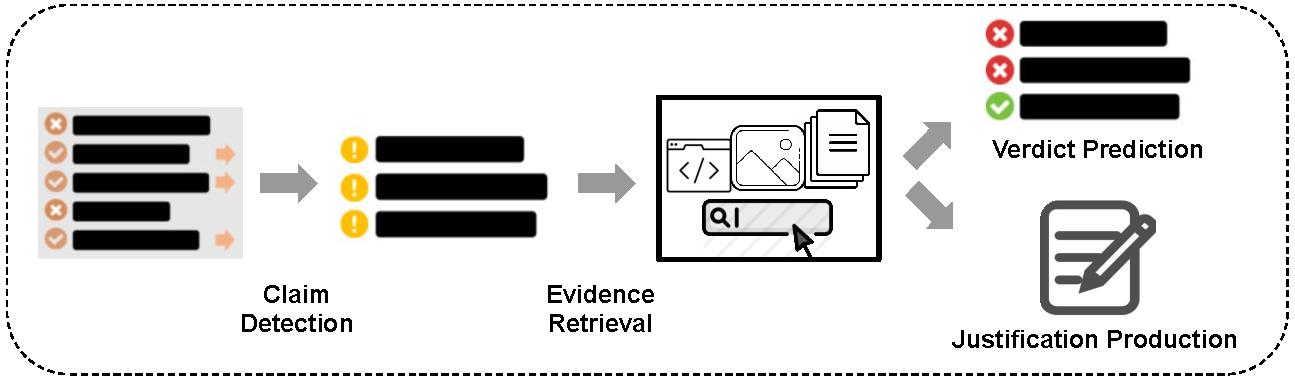
\includegraphics[width=14cm]{fig/framework.pdf}
    \caption{Automated fact-checking pipeline, reprinted from~\cite{guo-etal-2022-survey}}
    \label{fig:framework}
\end{figure}

Despite the existence of end-to-end fact-checking services, such as \url{politifact.org} or \url{demagog.cz}, the human-powered approach shows weaknesses in its scalability. By design, the process of finding an exhaustive set of evidence that decides the claim veracity is much slower than that of generating false or misguiding claims. Therefore, efforts have been made to move part of the load to a computer program that can run without supervision.

The common research goal is a fact verification tool that would, given a claim, semantically search provided knowledge base (stored for example as a \textit{corpus} of some natural language), propose a set of evidence (e. g. $k$ semantically nearest paragraphs of the corpus) and suggest the final verdict (Figure \ref{fig:pipeline}). This would reduce the fact-checker's workload to mere adjustments of the proposed result and correction of mistakes on the computer side. 

The goal of the ongoing efforts of {\textsf{FactCheck}} team at {\textsf{AIC CTU}}, as addressed in the works of~\cite{rypar,dedkova} and~\cite{gazo} is to explore the state-of-the-art methods used for fact verification in other languages, and propose a strong baseline system for such a task in Czech.


\section{A word on the Transformers}
\label{sec:transformers}
For the past six years, the state-of-the-art solution for nearly every Natural Language Processing task is based on the concept of \textit{transformer networks} or, simply, \textit{Transformers}. This has been a major breakthrough in the field by~\cite{vaswani}, giving birth to the famous models such as \textsf{Google}'s \textsf{BERT}~\cite{bert} and its descendants, or the \textsf{OpenAI}'s \textsf{GPT-3}~\cite{gpt3}.

In our proposed methods, we use Transformers in every step of the fact verification pipeline. Therefore, we would like to introduce this concept to our reader to begin with. 

Transformer is a neural model for \textit{sequence-to-sequence} tasks, which, similarly e.g. to the \textit{LSTM-Networks}~\cite{lstm}, uses the Encoder--Decoder architecture. Its main point is that of using solely the \textit{self-attention} mechanism to represent its input and output, instead of any sequence-aligned recurrence~\cite{vaswani}.

In essence, the \textit{self-attention} (also known as the \textit{intra-attention}) transforms every input vector to a weighted sum of the vectors in its neighbourhood, weighted by their \textit{relatedness} to the input. One could illustrate this on the \textit{euphony} in music, where every tone of a song relates to all of the precedent ones, to some more than to the others.

The full Transformer architecture is depicted in Figure~\ref{fig:transformer}.
%--- FIG: UTF forms
\begin{figure}
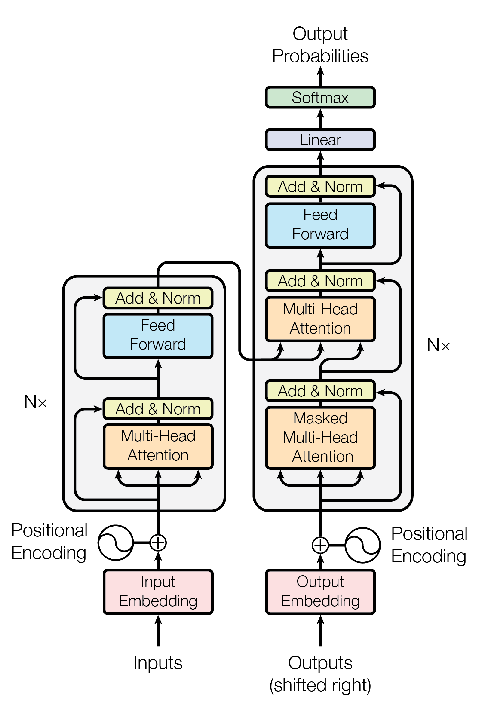
\includegraphics[width=9cm]{fig/transformer.pdf}
\caption{Transformer model architecture, reprinted from~\cite{vaswani}}
\label{fig:transformer}
\end{figure}
%--- /FIG



\section{Dissertation minimum study outline}
 
\begin{itemize}
\item {\techbf{Chapter~\ref{chap:intro}}} introduces the dissertation topic, motivates the research sets up our challenges for the future research 

\item {\techbf{Chapter~\ref{chap:sota}}} examines the most relevant research in the field and tries to highlight the recent paradigm shift from models trained for a single task to a single large models that perform well in everything

\item {\techbf{Chapter~\ref{chap:contribution}}} explains our current contributions to the field of automated fact-checking and NLP in Chech

\item {\techbf{Chapter~\ref{chap:plan}}} describes our plan for the dissertation and justifies the directions we are taking

\item Finally, {\techbf{Chapter~\ref{chap:conclusion}}} concludes the study with a wrapup of its findings

\end{itemize}


%!TEX ROOT=../ctutest.tex

\chapter{State of the Art}
%--- FIG: UTF forms

This chapter will first describe the originally popular models for general NLP, such as BERT and the recent paradigm shift from \textit{pretrain + finetune} transfer learning framework popular since the original~\cite{devlin2019bert} paper to the currently booming LLMs, which often outperform the smaller models even without the fine-tuning step~\cite{gpt4, llama, vicuna}. We will then take a look at the performance optimization methods that enable training multi-billion parameter pre-trained models on a set of task-specific data on a single GPU and their potential for our research. 

To show how it relates to our main topics, we will introduce currently published approaches for the automated fact-checking task, efforts related to claim generation, and evaluation of NLP model outputs.

\label{chap:sota}
\section{Pretrain + Finetune}
\label{sec:pretrain}
For the last decade, the \textit{pretrain-finetune} paradigm has been a cornerstone in Natural Language Processing (NLP). It has significantly shaped the development of modern NLP models. Its use in NLP can be traced back to the advent of neural networks and deep learning in the early 2010s. Initially, researchers pre-trained word embeddings using methods like Word2Vec~\cite{mikolov} and GloVe~\cite{pennington-etal-2014-glove}, which captured semantic relationships among words and then tweaked the general-task models for various related tasks.

\subsection{BERT and derivatives}\label{sec:bert}
The \textit{pretrain-finetune} paradigm truly rose to fame with the introduction of transformer-based models, particularly the revolutionary BERT (Bidirectional Encoder Representations from Transformers) in 2018. BERT~\cite{devlin2019bert} demonstrated the power of pretraining large-scale language models on massive text corpora using an easy-to-automate general task such as \textit{Masked Language Modeling}, or \textit{Next Sentence Prediction}, followed by fine-tuning on specific downstream tasks using smaller, harder-to-obtain data. This approach achieved state-of-the-art results across various NLP benchmarks. Subsequently, numerous variations of pre-trained models like GPT (Generative Pre-trained Transformer) and RoBERTa emerged, each refining the pretrain-finetune paradigm to improve language understanding, generation, and transfer learning capabilities. 

Importantly, BERT's success inspired many publications in training similar transformer models, varying in the definition of the general pre-training task, model size, architecture training corpus

\begin{itemize}
    \item In Czech language, monolingual models CZERT~\cite{czert}, FERNET~\cite{fernet}, RobeCzech~\cite{straka2021robeczech}, and small-e-czech~\cite{kocian2021siamese} are available for further finetuning
    \item In Polish, HerBERT~\cite{mroczkowski-etal-2021-herbert} achieved state-of-the-art in multiple tasks in 2021
    \item In Slovak, SlovakBERT~\cite{pikuliak2021slovakbert} was released by KInIT and Gerulata
    \item A multitude of multilingual models, such as \MBERT or \XLM~\cite{xlm-roberta} were pre-trained on data in all three of these languages (and many others), proving that the large transformers can capture a notion of semantics and relations between pieces of text even \textit{without} the convenient constriction of a single language 
\end{itemize}

\section{Few-shot and Zero-shot learning}
\label{sec:llms}
The ever-growing (sometimes billions of parameters in size) transformer models have not only demonstrated superior performance on benchmark datasets but have also shown remarkable zero-shot and few-shot learning abilities, where they can perform tasks with minimal or no task-specific training data~\cite{gpt3}.

Few-shot learning refers to the capability of a model to perform a task when provided with only a limited amount of labeled examples. Zero-shot learning takes this concept a step further by enabling models to tackle tasks they have never seen during training. The integration of these learning paradigms into large language models like GPT-3 and subsequent iterations has spread the NLP hype even further. By utilizing a prompt or a few examples, these models can quickly adapt to new tasks, making them highly versatile, adaptable, and usable to the general public.
\subsection{OpenAI LLMs: GPT-3 and GPT-4}
\label{sec:gpt}
In 2020, the few-shot learning was exhibited on GPT3 -- a 175B-parameter autoregressive model trained by~\cite{gpt3}. The model was trained on the task of generating text based on user's and its own previous outputs.
The training procedure and data\footnote{A mixture of crawled websites, books, and Wikipedia.} is thoroughly described in the publication. However, it is prohibitively costly for most labs to reproduce or even fine-tune at such a scale. 

In the fall of 2022, GPT-3 became widely popular thanks to its \textsf{ChatGPT}\footnote{\url{https://chat.openai.com}} fine-tune and demonstration app, which puts the user in the role of \textit{prompter}, texting back and forth with an LLM that predicts the most fitting reply to each conversation.

With the arrival of GPT-4, the \textsf{ChatGPT} was already massively famous, and the new model already shipped with a paid-service business scheme no longer publishing the training data, tasks, or even model size~\cite{gpt4}.

\section{Open source LLMs}
This puts the research community in an awkward position, as the GPT-4 achieves state-of-the-art in numerous NLP benchmarks~\cite{gpt4, Liu_2023}, but is designed not to be used in any way other than as a black box, making the derived research rigorosity and reproducibility disputable.

From the prediction times, \textsf{OpenAI} claims, and general trends in NLP, there are also reasons to believe that GPT-4 is orders of magnitude larger than already wasteful GPT-3.
This motivates an uptick in research of other LLMs that would be able to operate on a smaller scale with similar results, using a peer-reviewed architecture, training scheme, and data that is available in open source.

\subsection{LLaMA-2 and derivatives}
\label{sec:llama}

A popular foundational LLM to compete with the GPT family has become the \textsf{LLaMA}~\cite{llama} from \textsf{Meta research}. LLaMA was trained on about 5TB of publicly available textual data\footnote{To be specific, LLaMA was trained using an autoregressive language modeling task on a mixture of English CommonCrawl Corpus, C4~\cite{raffel2020exploring}, Github, Wikipedia, Gutenberg Project, Books3 corpus, ArXiv and Stack Exchange} mainly in English. 

It comes in various sizes between 7B and 65B parameters, achieving a SOTA among open-source solvers in various tasks and an unmatched performance in the field of single-GPU (7B and 13B) model sizes.
LLaMA proceeds to be used as a goto base model for a number of successful open-source chatbots such as Alpaca~\cite{alpaca}, Vicuna~\cite{vicuna}, and OpenAssistant~\cite{openassistant}.

The pre-trained LLaMA weights are, however, published under a restrictive license that prohibits republishing the model weights even after tuning its parameters, which limits its fine-tuners to publishing delta- or xor-weights that can not be properly used without \textsf{Meta}'s permission.

LLaMA-2~\cite{llama2} addresses this inconvenience (as well as delivers its own take on the \textit{chatbot} task), yielding an ideal strong base model for experimentation with any NLP task in 7B, 13B, and 70B sizes.
The only obstacle left in the way is the computational cost of fine-tuning across so many parameters.

%Open-source, freely usable.
%Often poor czech coverage 
%Quantizace, 4b, 8b, zlomek parametrů\cite{openassistant}

\subsection{LoRA and other optimization}\label{sec:lora}
To be able to fine-tune multi-billion-parameter models such as \textsf{LLaMA-2}~\cite{llama2} on a single TPU, successful approaches have been published to dramatically cut down the training expenses.
Parameter-efficient fine-tuning (PEFT)~\cite{peft} proposes approaches to only fine-tune \textit{a few} weights as opposed to the whole neural network, reducing the number of trainable parameters by orders of magnitude.
Low-Rank Adaptation of Large Language Models (LoRA)~\cite{lora} does so by freezing the pre-trained model weights and injecting trainable rank decomposition matrices into each layer of Transformer architecture. 

Quantization, which cuts the costs of working with 32- or 16-bit float parameters and opting for data types of bitsize as small as 4, also proves to be a powerful tool for LLM finetuning performance optimization~\cite{dettmers2023qlora}.
Quantized QLoRA takes LLaMA and finetunes it into a Guanaco model family, which outperforms all previous openly released LLMs on Vicuna benchmark~\cite{dettmers2023qlora} and achieves 99.3\% of the ChatGPT's performance on it while only requiring 24 hours on a single GPU.

As per an alleged leaked Google memo~\cite{moat}, this could put the future state of the art in NLP disciplines back into the hands of open source and public research, not giving any of the big tech companies a \"{moat} advantage.

Either way, it goes to show that the open-source LLMs have a promising future in NLP and will be indismissible as an approach for the NLP task of \textit{Automated fact checking}.

\section{Fact checking approaches}
Back in the late 2010s, the misinformation and its spread in the era of the internet and social media became a discussed topic in the Western world, with multiple institutions such as the European Council marking it a severe threat to democracy and national safety~\cite{disorder}.
The public attention and maturation of appropriate technologies motivated numerous efforts in business and academia to tackle the challenge.
Among other events, a Fake News Challenge occurred in 2017~\cite{fncweb} exploring the uses of technologies in the field and applying, for example, the LSTMs to detect stances among textual data~\cite{fnc}.

\subsection{FEVER and followups}
Soon, standard tasks began to be formulated and data collected. 
The FEVER (Fact Extraction and VERification)~\cite{fever} dataset and shared task became prominent in natural language processing research.
Relatively early on, it formalized the task as a two-step problem:
\begin{enumerate}
    \item Retrieving information within a structured corpus to fact-check a given claim (this resembles a standard NLP problem called \textit{information retrieval} -- IR)
    \item Classifying the inference relation between retrieved information and claim as one of:
    \begin{enumerate}
        \item {\techbf supports} -- information semantically implies the claim 
        \item {\techbf refutes} -- information semantically implies the negation of the claim 
        \item {\techbf not enough info} otherwise 
    \end{enumerate}
    This classification task became known as \textit{natural language inference} and mostly replaced the previous binary classification NLP task of \textit{recognizing textual entailment} (RTE)
\end{enumerate}

The FEVER dataset was a collection of 185K human-annotated claims, their veracity labels, and sets of evidence from a structured corpus that sufficed to justify the labels.
The corpus of choice was a 2017 English Wikipedia structured into articles due to its reasonable size, informational richness, and open license.\footnote{Is Wikipedia a trustworthy informational canon, though? 
No, it is not supposed to -- FEVER states that it is crucial to always maintain that the fact-checking classifiers only classify \textit{with respect to} data, and their reliability goes only as far as that of the underlying knowledge corpus. Therefore, \textit{supports} does not directly translate to \textit{true}, nor \textit{refutes} to \textit{false}}

FEVER yields an interesting benchmark with statistically quantifiable model success, motivated multiple well-performing public solutions~\cite{fever1,fever2}, gives insights into the complexities of automated fact-checking task, and strong baselines for research in the field. The data was later enriched by contrastive evidence in VitaminC~\cite{DBLP:journals/corr/abs-2103-08541} and by reasoning over tabular data in FEVEROUS~\cite{aly2021feverous}.

To date, it keeps being a reference point in automated fact-checking research despite its limitations, such as its requirement for a fixed knowledge base and \"{atomicity}\footnote{See section 4.1.2.\ref{atomicity}} of claims.

\begin{figure}
    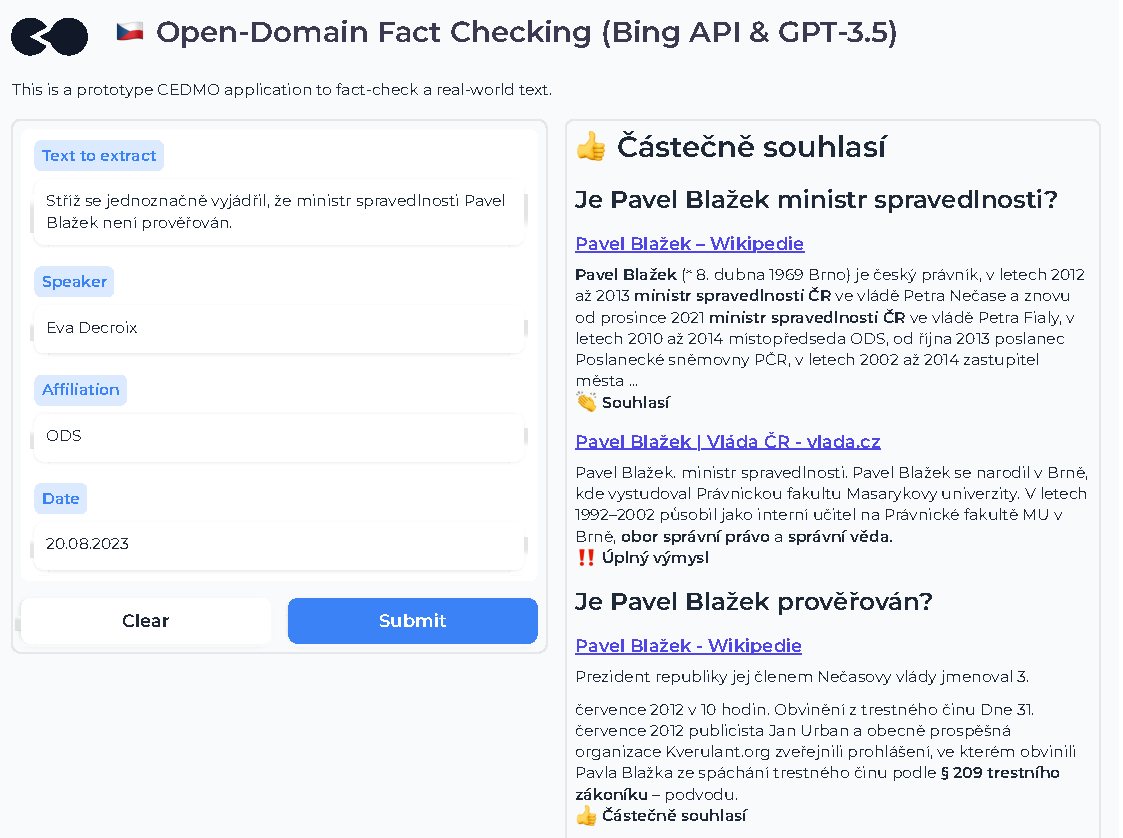
\includegraphics[width=14cm]{fig/bing.pdf}
    \caption{Proof-of-concept Czech fact-checking based on live-internet search (Bing API) and LLM prompting, based on the proposals of~\cite{bing} in Czech, using a real-world claim that was fact-checked by \href{https://demagog.cz/vyrok/22849}{\url{demagog.cz}} in June 2023}
    \label{fig:bing}
\end{figure}

\subsection{Open-domain fact-checking}
Due to these limitations, some researchers consider the scheme from FEVER an oversimplification -- the real politics' claims to be fact-checked by journalists often consist of long syntactical structures, combine information together in a non-trivial manner and often require the most up-to-date evidence. 

\"{Complex Claim Verification with Evidence Retrieved in the Wild}~\cite{bing} proposes a different scheme that overcomes these shortcomings:

\begin{enumerate}
    \item Arbitrarily complex claim is decomposed into a set of yes/no questions
    \item An open-domain search (Bing is proposed in the paper) fetches several evidence documents for each question
    \item A claim-focused summary is extracted from each document
    \item A veracity classifier goes through each pair of evidence and question, ranging from \"{faithful} to \"{completely wrong}
    \item The scores are combined (all need to be \"{faithful} for a faithful claim. Otherwise, the severity of inaccuracies can be approximated using some averaging.
\end{enumerate}

GPT-3 is used in steps 1, 3, and 4 of the scheme in the prototype delivered in~\cite{bing} in a few- and zero-shot fashion, with few-shot unsurprisingly coming out a little better. The scheme is transducible to Czech, and Figure~\ref{fig:bing} shows my early experiments with my interactive reproduction of it, predictors based on Bing and GPT-3.5 (a polished version of GPT-3).

While the shift from an established FEVER framework to complex real-world claims and evidence retrieval \"{in the wild} feels exciting and practical, an obvious pitfall arises -- anyone can publish anything on the internet, having it appear in Bing search and other crawlers alike. I argue that this might lead into a sort of a circular dependency of needing to reliably fact-check the evidence we have retrieved from the web in order to be able to build a reliable fact-checker in the first place.

Anyhow, the open-domain fact-checking idea opens a whole new range of approaches and shows the power of LLMs in fact-checking at its every step.

\section{Claim generation}
Another step of the fact-checking pipeline, covered by very few research publications, is the generation of the claim to be checked in the first place~\cite{guo-etal-2022-survey}.

The current state of things is that journalists who fact-check statements within, say, a Facebook status, need to read through the whole document multiple times, formulate its factual claims from the stances and facts expressed in the text themselves, and then fact-check each separately.

What has been examined so far were, for example:
\begin{itemize}
    \item Using Question Generation (QG) solver and converting the questions into declarative sentences to emulate more claims and more data for fact checking~\cite{pan2021zeroshot}
    \item Numerous CLEF CheckThat! challenges explored the task of estimating \textit{checkworthiness} of different parts of a long text, such as lines in a political debate~\cite{clef19,clef21}
    \item The task of extreme summarization (XSum) consists of summarizing a long body of text into a single sentence, focusing on its most relevant aspects and facts. Large datasets XSum~\cite{narayan-etal-2018-dont} in English and XL-Sum~\cite{xlsum} in 44 languages both present expertly annotated data from BBC News for it, as their article standard features a single-sentence summary at the beginning of each text.
\end{itemize}

\subsection{NLP summarization benchmarking}
\label{benchmarking-sota}
An important caveat to note with the NLP tasks reducing longer text to shorter text -- such as summarization or claim extraction -- is that the standard automatic metrics such as ROUGE~\cite{lin-2004-rouge} and METEOR~\cite{banerjee-lavie-2005-meteor} only focus on the \textit{content selection} aspect of tasks, based on a word-by-word overlap and were designed to use on multiple gold summaries per input, which are not often provided with modern large-scale datasets.~\cite{nlpprogress,bert-score,zha2023alignscore}

These serious limitations make it questionable for anyone to claim state-of-the-art on these tasks and motivate research for new metrics to cover all the important aspects of claim generation and do so in correlation with expert human judgment. 

This will be the topic of section~\ref{metrics}, which also introduces the state-of-the-art research we are working with to arrive to a valid set of benchmarks.
%!TEX ROOT=../ctutest.tex

\chapter{Current Contribution}
\label{chap:contribution}

\textit{We have collected novel data for the fact-checking task in our application context, emulated and scraped inavailable datasets making them public or readying them for doing so, we have established numerous state-of-the-art models and we are currently working on establishing the topic of claim generation as a summarization-related NLP task.}

\section{Datasets}
Having the automated fact-checking scheme established in chapter~\ref{chap:sota}, every machine-learning solution must start with the choice or collection of appropriate training data.
Due to the novelty of the task in Czech and other West Slavic languages, I explored a multitude of ways to acquire such data, many of them resulting in a publicly available dataset in our Huggingface repository~\footnote{\url{https://huggingface.co/ctu-aic}}, beginning to be reused by others. 

\subsection{\FCZ}\label{sec:fcz}
An early \"{temporary benchmark} for our endeavours in adapting the FEVER~\cite{fever} task for the Czech context was the \FCZ~\cite{lrev} dataset.

In~\cite{diplomka}, I have proposed a simple FEVER data transduction scheme that can be simplified as follows:

\begin{enumerate}
    \item Each FEVER claim is translated using the (at the time maturing) Machine Translator
    \item Evidence from English Wikipedia is not translated using MT, but mapped onto its Czech-Wikipedia counterpart using the publicly available Wikidata\footnote{Used, for example, for showing the \"{see this article in other languages} suggestions in Wikipedia sidebar}
    \item Data with any loss in evidence due to the step 2. is discarded
\end{enumerate}

This design was relatively cheap to compute (as translating the whole 2017 Wikipedia corpus would have been a long and wasteful computation), delivering an open-license dataset of 127K claims, their labels and evidence justifications. My hope was, as both the 2017 EnWiki and our 2020 CsWiki corpus only featured the first paragraph (abstract) of each article, a document-level alignment could be assumed -- both the Czech and English text always summarize the basic facts about the same entity.

This showed to be only partly true as a later human annotation on a 1\% sample of \FCZ data showed that about a third of data exhibits some levels of noise, mostly introduced during dataset translation~\cite{lrev}.

While noisy, the \FCZ data still got its use in training of the information retrieval schemes of~\cite{rypar,gazo,lrev} used to this day and is openly available\footnote{\url{https://huggingface.co/datasets/ctu-aic/csfever}} under a CC license.

My research on it also motivated a creation of a inference-only version of the dataset, which does not support the Information Retrieval task and therefore, does not require the mapping of evidence into a live version of Wikipedia.
Therefore, only the EnWiki \textit{excerpts} needed to build evidence can be translated, bringing down the computational difficulty and enabling me to deliver a dataset without the transduction noise called \FCZNLI\footnote{\url{https://huggingface.co/datasets/ctu-aic/csfever_nli}}. 

Another round of research \FCZ motivated and I supervised was the successful thesis of~\cite{mlynar}, modernizing the data and machine-translation methods into the 2023 state of the art.
\cite{mlynar} further experimented with methods of automated noise detection and removal, which has not shown to be an efficient way to tackle the issue of high noise in \FCZ.

However, it delivers a partly cleaned versions of it\footnote{\url{https://huggingface.co/datasets/ctu-aic/csfever_v2}} and motivates a future research of generating such data differently, using a claim generation scheme like that from~\cite{pan2021zeroshot}.


\subsection{FCheck Annotations Platform}
The imperfections in translated \FCZ data, as well as the ongoing colaboration with ČTK and the Faculty of Social Sciences brought me to also look for ways how to hand-annotate a whole new natively Czech dataset, which would both lack the noise of translated data and take the task of automated fact checking to next level, replacing a rigid, simple Wikipedic data with a more \"{real world} news report corpus of ČTK.

Figure~\ref{fig:fcheck} shows an open-source platform FCheck\footnote{\url{https://fcheck.fel.cvut.cz} (\texttt{testuser}), source at: \href{https://github.com/aic-factcheck/fcheck-annotations-platform}{\texttt{github.com/aic-factcheck/fcheck-annotations-platform}}} I developed to collaborate with 316 FSV CUNI students of on a collection of novel dataset in Czech using ČTK data as a ground truth corpus.
\label{sec:datasets}
\begin{figure}[H]
    \makebox[\textwidth][c]{
    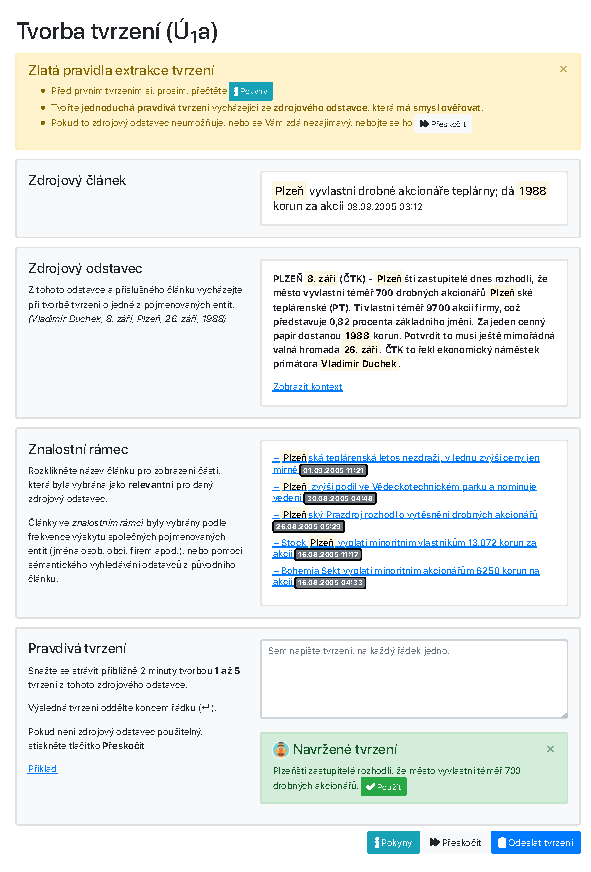
\includegraphics[height=7.5cm]{fig/fcheck/claim_extraction.pdf}
    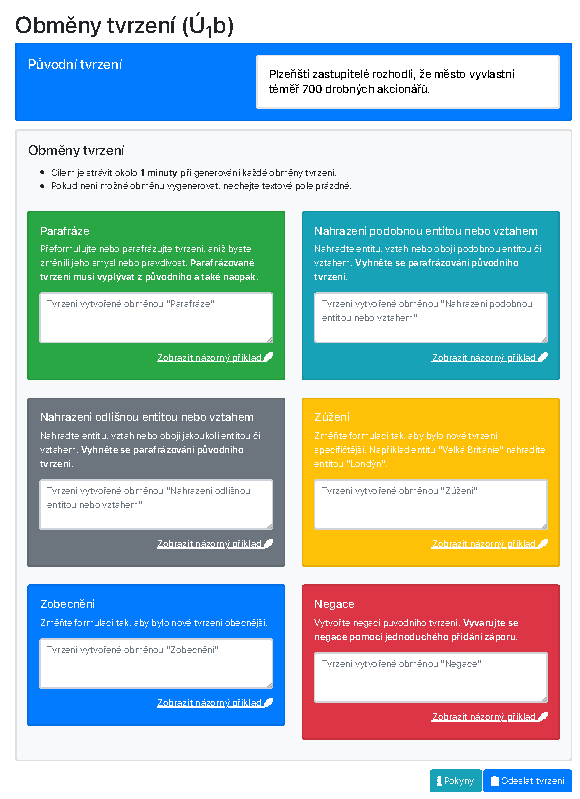
\includegraphics[height=7.5cm]{fig/fcheck/mutation.pdf}
    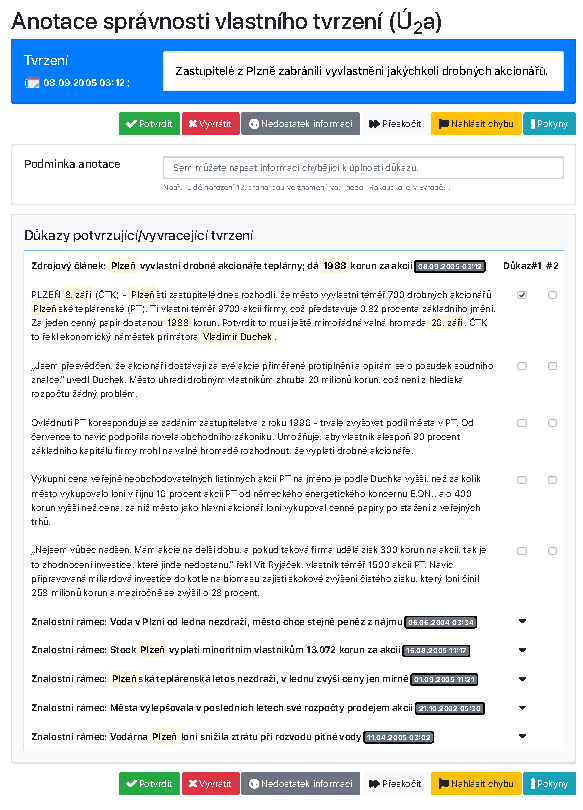
\includegraphics[height=7.5cm]{fig/fcheck/annotation.pdf}
    }
    \caption{{\techbf FCheck} -- platform for fact-checking data collection developed for TAČR project; collects data for claim generation, information retrieval and natural language inference tasks}
    \label{fig:fcheck}
\end{figure}

We have established a 4-step annotation procedure inspired by the time-proven methodology of~\cite{fever} where chech-worthy paragraphs are first hand-picked among samples from the whole archive of ČTK's 3.3 M news reports published between 1 January 2000 and 6 March 2019. Then, the annotator is sampled such a paragraph and asked to \textit{extract claims} from it, i.e., formulate single-sentence summaries of some facts that appear in paragraph. This claim is always \textit{supported} by the data, so the next phase is to perturb the claim by annotator's world knowledge and form the claim \textit{mutations} -- substitutions of entities, generalizations, specifications, paraphrases or negations of the original claim. 
The mutated claim is then fact-checked by (typically) another annotator, using the ČTK data narrowed down to a reasonable number of relevant articles (in an IR sense) as \textit{supportable}, \textit{refutable} or \textit{not enough info}, providing a set of evidence as a verdict justification.

The whole application is running on multiple levels -- a yii-framework-powered PHP app is running the annotation interface, while a flask server in python is running our models based on TF-IDF~\cite{drqa} and mBERT (section~\ref{sec:bert}) for information retrieval trained among other data on the \FCZ dataset (section~\ref{sec:fcz}).
The models are solving the Information Retrieval task on-demand (with cache) on the proprietary ČTK corpus, whenever the annotation app needs it to provide a context to the fact-checker.

The scheme and its implementations are exhaustively described in~\cite{diplomka}, chapter 4 and in~\cite{lrev}, also chapter 4.
Multiple \"{cross-annotations} were collected for each claim, to measure agreement and give insights into task complexity.

\subsection{\CTK}
\label{sec:ctkfacts}


After completing the first year of annotation experiments, we have extracted a total of 3,116 multi-annotated claims.
47\% were \texttt{SUPPORT}ed by the majority of their annotations, \REF{} and \NEI{} labels were approximately even, the full distribution of labels is listed in Table~\ref{tab:ctkfacts}.
% We have originally experimented with balanced \dev and \test splits to punish predictors exploiting this bias.

\begin{table}[H]
    \makebox[\textwidth][c]{
    \begin{ctucolortab}
    \begin{tabular}{ r || ccc || ccc  }
    &  \multicolumn{3}{c}{\techbf{{\CTK}}} uncleaned, balanced & \multicolumn{3}{c}{\techbf{{\CTK}} (launch)} cleaned, stratified\\
    \hline
    {} & {\texttt{SUPPORTS}} & \texttt{REFUTES}  & \texttt{NEI} & {\texttt{SUPPORTS}} & \texttt{REFUTES}  & \texttt{NEI}\\ 
    \hline
    \train  & 1,164 & 549 & 503     & 1,104 & 556 & 723 \\
    \dev    & 100 & 100 & 100       & 142 & 85 & 105\\
    \test   & 200 & 200 & 200       & 176 & 79 & 127\\
    \end{tabular}
    \end{ctucolortab}}
    \caption{Label distribution in \CTK splits before and after cleaning. Reprinted from~\cite{lrev}}
    \label{tab:ctkfacts}
    \end{table}

Of all the annotated claims, 1,776, that is 57\%, had at least two independent labels assigned by different annotators.
I used this multiplicity to asses the quality of our data and ambiguity of the task, as well as to propose annotation cleaning methods used to arrive to our final \text{cleaned} \CTK dataset.

\subsubsection{Inter-Annotator Agreement}
\label{sec:agreement}

Due to our cross-annotation design, I had generously sized sample of independently annotated labels in our hands.
As the total number of annotators was greater than 2, and as missing observations were allowed, I have used the Krippendorff's alpha measure~\cite{krippendorff1970} which is the standard for this case~\cite{hayes2007krippendorff}.
For the comparison with \cite{fever} and \cite{norregaard2021danfever}, I also list a 4-way Fleiss' $\kappa$-agreement~\cite{fleiss1971measuring} calculated on a sample of 7.5\% claims.

I have calculated the resulting Krippendorff's alpha agreement to be 56.42\% and Fleiss' $\kappa$ to be 63\% and interpreted this as an adequate result that testifies to the complexity of the task of news-based fact verification within a fixed knowledge scope.
It also encourages a round of annotation cleaning experiments that would exploit the number of cross-annotated claims to remove common types of noise.

\subsubsection{\CTK publication}
\CTK dataset was then subject to a thorough human-in-the-loop data cleaning until a 100\% agreement among the data was reached, in order to remove data that contains obvious noise and reveal phenomena that lead to erroneous annotations.
The full process as well as it results are described in~\cite{lrev}.

Ultimately, a dataset of 3.1K thorougly cleaned data points in a form of a factual claim, its veracity label and justifications consisting of ČTK paragraphs was published in a version for Information Retrieval\footnote{\url{https://huggingface.co/datasets/ctu-aic/ctkfacts}} for those who have access to the ČTK knowledge base to retrieve from, as well as in a special version for the task of Natural Language Inference\footnote{\url{https://huggingface.co/datasets/ctu-aic/ctkfacts_nli}} containing all the required ČTK excerpts we have negotiated to publish under open license for everyone to use.

The datasets have become our standard benchmark within the AIC NLP group~\cite{semin,mlynar} and are starting to be referred and used in others' research in the field~\cite{stefanik}.

\subsection{Other NLP datasets in West Slavic languages}
Over the time, we have accumulated numerous sets of data in Czech and other Slavic languages that have previously been poorly covered or not available at all, some of which are to be referred in our future publications.
For the convenience of others, most of them are already listed in our public repositories.
Let us mention some significant examples:

\begin{enumerate}
    \item We have machine-translated the most popular NLI training and benchmark datasets such as Stanford NLI~\cite{snli:emnlp2015}, Adversarial NLI~\cite{anli} and MultiNLI~\cite{multinli} picking a machine translator empirically for each dataset between DeepL~\cite{deepl}, Google Translate~\cite{googletranslation} and CUBBITT~\cite{popel2020Transforming}.
    
    The resulting datasets can are maintained at our public repositories:
    \begin{enumerate}
        \item \url{https://huggingface.co/datasets/ctu-aic/snli_cs}
        \item \url{https://huggingface.co/datasets/ctu-aic/anli_cs}
        \item \url{https://huggingface.co/datasets/ctu-aic/multinli_cs}
    \end{enumerate}
    \item For the task of claim generation we are establishing and performing in Czech, we have adapted the existing related datasets and are working with:
    \begin{enumerate}
        \item CTKSum -- \url{https://huggingface.co/datasets/ctu-aic/ctksum} based on source articles and extracted claims within the original \CTK{} set
        \item FEVERSum (based on FEVER Wikipedia abstract and extracted claims) -- \url{https://huggingface.co/datasets/ctu-aic/fever-sum}
        \item Its DeepL translation CsFEVERSum -- \url{https://huggingface.co/datasets/ctu-aic/csfever-sum}
        \item Our reproduction of a crawled Slovak summarization dataset described by~\cite{suppa-adamec-2020-summarization} SMESum based on articles from \url{https://sme.sk} -- \url{https://huggingface.co/datasets/ctu-aic/smesum}
    \end{enumerate}
\end{enumerate}
Up until now, some of the data was restricted to private repositories, but with this study, I am publishing most of them, as I have now found the licensing to be rather relaxed.
If some of the repositories reader might be interested in would not be reachable, please request access to the  \url{https://huggingface.co/datasets/ctu-aic} organization to be able to see into the private part of our dataset library.

\section{Models}
\label{sec:models}
The most significant pretrained models I have made public address two tasks -- the Natural Language Inference and Claim Generation viewed as a form of Abstractive Summarization task.
\subsection{Natural Language Inference}
My previous work~\cite{diplomka, lrev} also focused on establishing a strong starting state of the art on our own datasets in the tasks of NLI.
In my publications, I have tried and compared a multitude of neural networks for the tasks, ultimately arriving to:
\begin{itemize}
    \item {\techbf XLM-RoBERTA-Large@XNLI@\FCZNLI}, a model with 561M parameters trained on 100-language CommonCrawl corpus finetuned on multilingual XNLI~\cite{conneau2018xnli} inference datased and then finetuned \textit{again} on the \FCZNLI task yields an unmatched 73.7\% F1 macro score on the denoised \FCZNLI inference task: \url{https://huggingface.co/ctu-aic/xlm-roberta-large-xnli-csfever_nli}
    \item {\techbf XLM-RoBERTA-Large@SQuAD2}, a model version finetuned on a Question answering SquAD2~\cite{squad} task has shown remarkable practicality in my NLI applications and after task specific finetuning, it was able to tackle:
    \begin{enumerate}
        \item \CTKNLI\footnote{\url{https://huggingface.co/ctu-aic/xlm-roberta-large-squad2-ctkfacts_nli}} task with 76.9\% macro-F1
        \item \FCZ\footnote{\url{https://huggingface.co/ctu-aic/xlm-roberta-large-squad2-csfever_nearestp}} (noisy) task with 83.2\% macro-F1
        \item The original English FEVER NLI task\footnote{\url{https://huggingface.co/ctu-aic/xlm-roberta-large-squad2-enfever_nli}}~\cite{fever,nie2019combining}, achieving 75.9\% macro-F1 and a significant superiority over previous shared task winner~\cite{nie2019combining} (which had 69.5 macro-F1 with NSMNs)
    \end{enumerate}
\end{itemize}

\subsection{Claim generation}
In my current research, I am finding appropriate configurations and data to train models for the task of claim generation -- generating a factual claim (or more) into a single sentence that contains a fluent, atomic, decontextualized and faithful claim.
In section~\ref{generation}, I~propose the claim generation as an abstractive summarization setting, and therefore, the models already have their practical use in the general task of summing up longer texts into shorter ones.

As has been shown in section~\ref{benchmarking-sota}, NLP summarization task does not have a reliable standard benchmark that would capture all its required output qualities. Therefore, it remains questionable to claim the state of the art on any summarization task and I proceed to present models that excel in our empirical tests and demonstrations for project stakeholders:

\begin{enumerate}
    \item {\techbf mBART}~\cite{mbart} multilingual Transformer model has been finetuned by our team's~\cite{krotil} on SumeCzech and proprietary CNC News summarization dataset on the \"{full text to headline} task, obtaining encouraging scores across numerous summarization metrics in Czech.\\
    I have taken this model a step further for the claim generation task, finetuning it on the {\FCZ}Sum and {\CTK}Sum datasets, yielding a working model for the task.\footnote{
    \url{https://huggingface.co/ctu-aic/mbart25-large-eos}}

    Another experiments are being carried out with the same model finetuned on Slovak\footnote{\url{https://huggingface.co/ctu-aic/mbart-at2h-cs-smesum-2}} and Polish\footnote{\url{https://huggingface.co/ctu-aic/mbart-at2h-cs-polish-news3}} data.
    \item {\techbf LLaMA-2} shows promissing result when it comes to claim generation.
    I have finetuned\footnote{\url{https://huggingface.co/ctu-aic/Llama-2-7b-xlsum-en}} it using the QLoRA (section~\ref{sec:lora}) approach, XL-Sum~\cite{xlsum} dataset and a concatenation-based prompting strategy~\cite{llama2}, to facilitate training across the entire length of input.
    
\end{enumerate}

All prototype models are currently being iterated with our CEDMO project partners (fact-checkers from European organizations),  tweaked, and future tests are being designed for them based on empirical results and questionnaires.


\section{Applications}
\label{sec:applications}
Several applications demonstrating our contributions are currently deployed and available online due to the CEDMO project and their testing with future users, let us therefore present the main applications I and my supervisor Jan Drchal have developed for the tasks:

\begin{enumerate}
    \item Claim extractor at \url{https://fcheck.fel.cvut.cz:1830} (figure~\ref{fig:claimgencedmo}) demonstrates the single or multiple claim generation task with our LLaMA-2 or mBART models for English and Czech texts, respectively, using a GRADIO interactive application and an API
    \item  \url{https://fcheck.fel.cvut.cz:1831} runs a FactSearch platform by Jan Drchal, demonstrating our best performing models for the whole fact-checking tasks, integrating the XLM-RoBERTas trained on \FCZNLI data
    \item  \url{https://fcheck.fel.cvut.cz:1832} runs the same scheme with our best performing English models and data
\end{enumerate}

\begin{figure}
    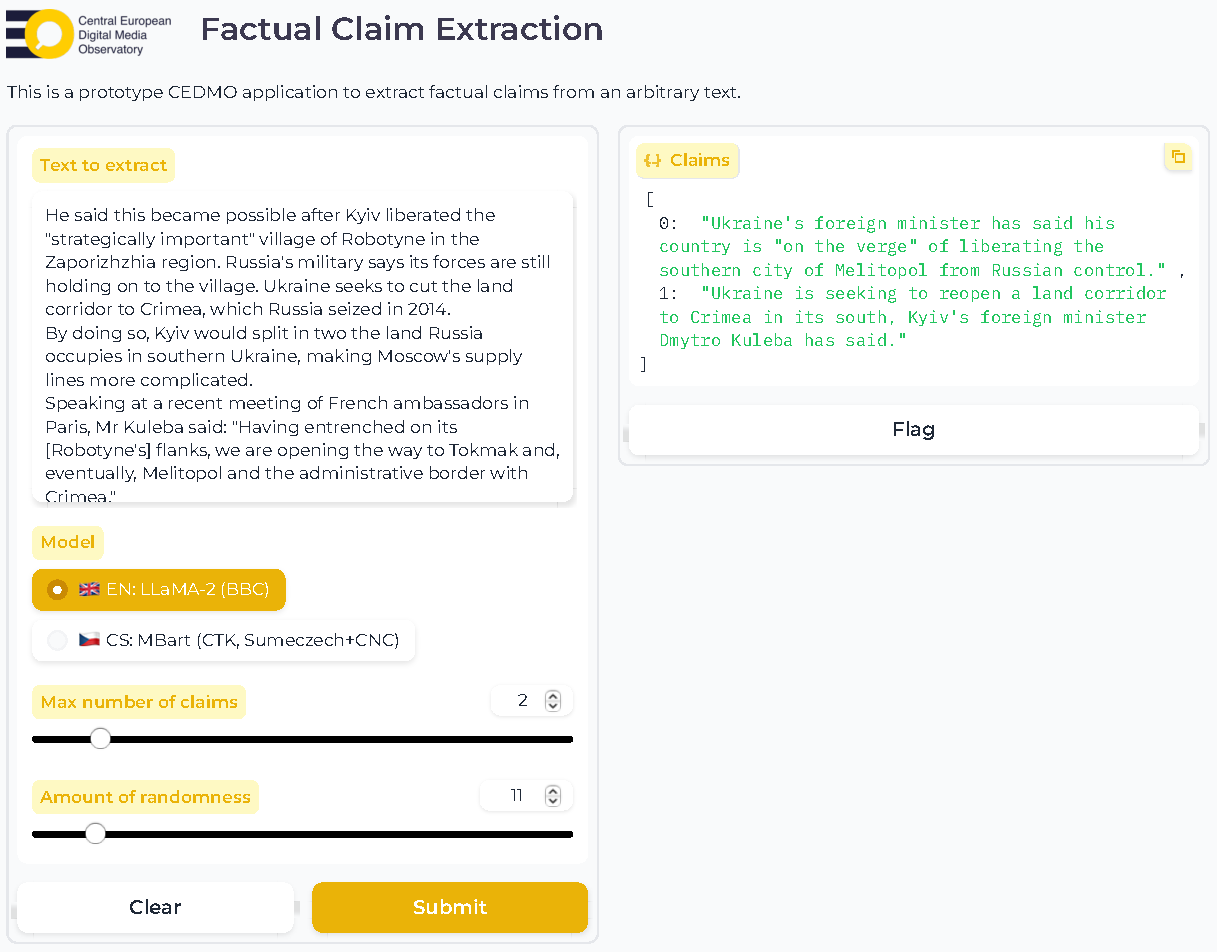
\includegraphics[width=16cm]{fig/cedmo.pdf}
    \caption{Factual claim extraction application done for the CEDMO project}
    \label{fig:claimgencedmo}
\end{figure}

Here we will show off the demonstration tools, as well as our open-source platform \url{https://fcheck.fel.cvut.cz} and currently running claim extraction tools. 
%!TEX ROOT=../ctutest.tex

\chapter{Dissertation plan}
\label{chap:plan}

%!TEX ROOT=../dissertation.tex

\chapter{AVeriTeC Paper}
\section{Introduction}
\label{sec:introduction}
We release \review{a} pipeline for fact-checking claims using evidence retrieved from the web consisting of two modules -- a \textit{retriever}, which picks the most relevant sources among the available knowledge store\footnote{Due to the pre-retrieval step that was used to generate knowledge stores, our \say{retriever} module could more conventionally be referred to as a \say{reranker}, which we refrain from, to avoid confusion with reranking steps it uses as a subroutine.} and an \textit{evidence \& label generator} which generates evidence for the claim using these sources, as well as its veracity label. 

Our pipeline is a variant of the popular Retrieval-augmented Generation (RAG) scheme~\cite{rag}, making it easy to re-implement using established frameworks such as Langchain, Haystack, or our attached Python codebase for future research or to use as a baseline.

This paper describes our pipeline and the decisions taken at each module, achieving a simple yet efficient RAG scheme that improves dramatically across the board over the baseline system from~\cite{averitec2024}, and scores third in the \averitec{} leaderboard as of August 2024, with an \averitec{} test set score of 50.4\%.

% show figures/pipeline.png
\begin{figure}[h]
    \centering
    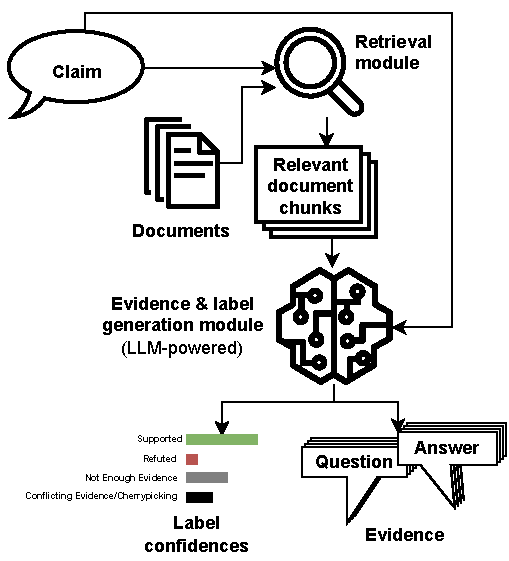
\includegraphics[width=0.47\textwidth]{figures/pipeline.pdf}
    \caption{Our pipeline}
    \label{fig:pipeline}
\end{figure}

\section{Related work}
\label{sec:relwork}
\label{avscore}
\begin{enumerate}
    \item \textbf{\averitec{} shared task}~\cite{averitec2024} releases the datase of real-world fact-checked claims, annotated with evidence available at the date the claim was made.
    
    \review{It proposes the \textbf{\averitec{} Score} -- a method of unsupervised scoring of fact-checking pipeline against this gold data using Hungarian METEOR score, matching the evidence questions (Q) or the whole evidence (Q+A).
    The score is then calculated as the proportion of claims with accurate label and sound evidence (using a threshold for Hu-METEOR such as 0.25) among all claims in the dataset, giving an estimate on \say{how often the whole fact-checking pipeline succeeds end to end}.}

    The provided \textbf{baseline} is a pipeline of search query generation, API search (producing a knowledge store), sentence retrieval, Question-and-answer (QA) generation, QA reranking, QA-wise claim classification and label aggregation, achieving an overall \averitec{} test set score of 11\%.  
    \item \review{\textbf{FEVER Shared Task}~\cite{thorne-etal-2018-fact}, a predecessor to the \averitec{}, worked with a similar dataset engineered on top of the enclosed domain Wikipedic data rather than real-world fact-checks. 
    Its top-ranking solutions used a simpler pipeline of Document Retrieval, Sentence Reranking and Natural Language Inference, improving its modules in a decoupled manner and scoring well above 60\% in a similarly computed FEVER score~\cite{thorne-etal-2018-fever} on this data.}
    \item \textbf{Our previous research} on fact-checking pipelines~\cite{Ullrich2023,drchal2023pipelinedatasetgenerationautomated} using data similar to FEVER and \averitec{} shows significant superiority of fact-checking pipelines that \textbf{retrieve the whole documents} for the inference step, rather than retrieving out-of-context sentences.
    \item \textbf{Retrieval-Augmented Generation (RAG) for Knowledge-Intensive Tasks}~\cite{rag} takes this a step further, leveraging Large Language Model (LLM) for the task, providing it the whole text of retrieved documents (each a chunk of Wikipedia) and simply instructing it to predict the evidence and label on top of it, achieving results within 4.3\% from the FEVER state of the art by the time of its publication (December 2020) \textit{without} engineering a custom pipeline for the task.
\end{enumerate}


\section{System description}
\label{sec:system}
\review{Our system design prioritizes simplicity, and its core idea is using a straightforward RAG pipeline without engineering extra steps, customizing only the retrieval step and LLM prompting } (Listing~\ref{lst:llm_system_prompt} \review{in Appendix~\ref{appendix_sec:system_prompt}}).
Despite that, this section describes and justifies our decisions taken at each step, our additions to the naive version of RAG modules to tune them for the specific task of fact-checking, and their impact on the system performance.

\subsection{Retrieval module}
\label{retrieval}
To ease comparison with the baseline and other systems designed for the task, our system does not use direct internet/search-engine access for its retrieval, but an \averitec{} \textit{knowledge store} provided alongside each claim.

\review{To use our pipeline in the wild, our retrieval module is decoupled from the rest of the pipeline and can be swapped out in favour of an internet search module such as SerpApi\footnote{\url{https://serpapi.com/}} as a whole, or it can be used on top of a knowledge store emulated using large crawled corpora such as CommonCrawl\footnote{\url{https://commoncrawl.org/}} and a pre-retrieval module.}

\subsubsection{Knowledge stores}
Each claim's knowledge store contains pre-scraped results for various search queries that can be derived from the claim using human annotation or generative models.
The knowledge stores used with ours as well as the baseline system can be downloaded from the \averitec{}  dataset page\footnote{\url{https://fever.ai/dataset/averitec.html}}, containing about 1000 pre-scraped \textit{documents}\footnote{\label{devsetnote}The numbers are orientational and were computed on knowledge stores provided for the \averitec{}  dev set.}, each consisting of $28$ sentences at median\footnoteref{devsetnote}, albeit varying wildly between documents.
The methods used for generating the knowledge stores are explained in more detail by~\citet{averitec2024}.
%To use our system in the wild, this knowledge store can be emulated using a search API such as SerpApi, or even a large document collection such as Common Crawl pruned down to similar orders of magnitude using a cheap retrieval method and the claim as a search query.

Our retrieval module then focuses on picking a set of $k$ ($k=10$ in the examples below, as well as in our submitted system) most appropriate document chunks to fact-check the provided claim within this knowledge store.

\subsubsection{Angle-optimized embedding search}
\label{sec:knn}
Despite each article in any knowledge store only needing to be compared \textit{once} with its \textit{one specific} claim, which should be the use-case for CrossEncoder reranking~\cite{dejean2024thoroughcomparisoncrossencodersllms}, our empirical preliminary experiments made us favour a \textit{cosine-similarity} search based on vector embeddings instead.
It takes less time to embed the whole knowledge store into vectors than to match each document against a claim using crossencoder, and the produced embeddings can be re-used across experiments.

For our proof of concept, we explore the MTEB~\cite{muennighoff-etal-2023-mteb} benchmark leaderboard, looking for a reasonably-sized open-source embedding model, ultimately picking Mixedbread's mxbai-large-v1~\cite{li-li-2024-aoe,emb2024mxbai} optimized for the cosine objective fitting our inteded use.

\review{To reduce querying time at a reasonable exactness tradeoff, we use Faiss index~\cite{douze2024faiss,johnson2019billion} to store our vectors, allowing us to only precompute semantical representation once, making the retriever respond rapidly in empirical experiments, allowing a very agile prototyping of novel methods to be used.}
\
\subsubsection{Chunking with added context}
Our initial experiments with the whole \averitec{}  documents for the Document Retrieval step have revealed a significant weakness -- while most documents fit within the input size of the embedding model, outliers are common, often with \textit{hundreds of thousands} characters, exceeding the 512 input tokens with little to no coverage of their content.

Upon further examination, these are typically PDF documents of legislature, documentation and communication transcription -- highly relevant sources real fact-checker would scroll through to find the relevant part to refer. 

This workflow inspires the use of \textit{document chunk retrieval} as used in~\cite{rag}, commonly paired with RAG.
We partition each document into sets of its sentences of combined length of $N$ characters at most.
To take advantage of the full input size of the vector embedding model we use for semantical search, we \review{arbitrarily} set our bound $N=512*4=2048$, \review{where 512 is} the input dimension of common embedding models, 4 often being used as a rule-of-thumb number of characters per token for US English in modern tokenizers~\cite{tokens}.

Importantly, each chunk is  assigned metadata -- the source URL, as well as the full text of the next and previous chunk within the same document.
This way, chunks can be presented to the LLM along with their original context in the generation module, where the length constraint is much less of an issue than in vector embedding.
As shown in~\cite{drchal2023pipelinedatasetgenerationautomated}, fact-checking models benefit from being exposed to larger pieces of text such as paragraphs or entire documents rather than out-of-context sentences.
Splitting our data into the maximum chunks that fit our retrieval model and providing them with additional context may help down the line, preventing the RAG sources from being semantically incomplete.

\subsubsection{Pruning the chunks}
While the chunking of long articles prevents their information from getting lost to retriever, it makes its search domain too large to embed on demand.
As each of the thousands of claims has its own knowledge store, each of possibly tens of thousands of chunks, we seek to omit the chunks having little to no common tokens with our claim using an efficient BM25~\cite{bm25} search for the nearest $\omega$ chunks, setting the $\omega$ to 6000 for dev and 2000 for test claims. 
This yields a reasonably-sized document store for embedding each chunk into a vector, taking an average of 40 s to compute and store using the method described in Section~\ref{sec:knn} for each dev-claim using our Tesla V100 GPU.

This allows a quick and agile production of vectorstores for further querying and experimentation, motivated by the \averitec{}  test data being published just several days before the announced submission deadline.
\review{The pruning also keeps the resource intensity moderate for real-world applications.
However, if time is not of the essence, the step can be omitted.}

\subsubsection{Diversifying sources: MMR}
\review{Our choice of embedding search based on the entire claim rather than generating \say{search queries} introduces less noise and captures the semantics of the whole claim.
It is, however, prone to redundancy among search results, which we address using a reranking by the results' Maximal Marginal Relevance (MMR)~\cite{carbonell-mmr}, a metric popular for the RAG task, which maximizes the search results' score computed as (for $D_i\in P$)
$$\lambda \cdot \mathrm{Sim}(D_i, Q) - (1-\lambda) \cdot \max_{D_j \in S} \mathrm{Sim}(D_i, D_j)$$
$Sim$ denoting the cosine-similarity between embeddings, $Q$ being the search query, and $P$ the pre-fetched set of documents (by a search which simply maximizes their $Sim$ to $Q$), forming $S$ as the final search result, by adding each $D_i$ as MMR-argmax one by one, until reaching its desired size.}

In our system, we set $\lambda=0.75$ to favour relevancy rather than diversity, $|S|=10$ and $|P| = 40$, obtaining a set of diverse sources relevant to each claim at a fraction of cost and complexity of a query-generation driven retrieval, such as that used in~\cite{averitec2024}.

\subsection{Evidence \& label generator}
\label{sec:generation}
The second and the last module on our proposed pipeline for automated fact checking is the Evidence \& Label Generator, which receives a claim and $k$ sources (document chunks), and returns $l$ (in our case, $l=10$) question-answer pairs of evidence abstracted from the sources, along with the veracity verdict -- in \averitec{} dataset, a claim may be classified as \textit{Supported}, \textit{Refuted}, \textit{Not Enough Evidence}, or \textit{Conflicting Evidence/Cherrypicking} with respect to its evidence.

Our approach leverages a Large Language Model (LLM), instructing it to output both evidence and the label in a single step, as a chain of thought.
We rely on JSON-structured output generation with source referencing using a numeric identifier, we estimate the label confidences using Likert-scale ratings.
The full system prompt can be examined in Listing~\ref{lst:llm_system_prompt} \review{in Appendix~\ref{appendix_sec:system_prompt},} and this section further explains the choices behind it.

\subsubsection{JSON generation}

To be able to collect LLM's results programmatically, we exploit their capability to produce structured outputs, which is on \review{the} rise, with datasets available for tuning~\cite{tang2024strucbenchlargelanguagemodels} and by the time of writing of this paper (August 2024), systems for strictly structured prediction are beginning to be launched by major providers~\cite{json}.

Despite not having access to such structured-prediction API by the time of \averitec{} shared task, the current generation of models examined for the task (section~\ref{sec:chosen_llms}) rarely strays from the desired format if properly explained within a system prompt -- we instruct our models to output a JSON of pre-defined properties (see prompt Listing~\ref{lst:llm_system_prompt} \review{in Appendix~\ref{appendix_sec:system_prompt}}) featuring both evidence and the veracity verdict for a given claims.

Although we implement fallbacks, less than 0.5\% of our predictions \review{threw} a parsing exception throughout experimentation, and could be easily recovered using the same prompting again, exploiting the intrinsic randomness of LLM predictions.

\subsubsection{Chain-of-thought prompting}
While JSON dictionary should be order-invariant, we can actually exploit the order of outputs in our output structure to make LLMS like GPT-4o output better results~\cite{cot}.
This is commonly referred to as the \say{chain-of-thought} prompting -- if we instruct the autoregressive LLM to first output the evidence (question, then answer), then a set of all labels with their confidence ratings (see section~\ref{likert}) and only then the final verdict, its prediction is both cheaper as opposed to implementing an extra module, as well as more reliable, as it must attend to all of the intermediate steps as well.

\subsubsection{Source referring}
To be able to backtrack the generated evidence to the urls of the used sources, we simply augment each question-answer pair with a source field.
We assign a 1-based index\footnote{\review{We chose the 1-based source indexing to exploit the source-referring data in LLM train set such as Wikipedia, where source numbers start with 1. The improvement in quality over 0-based indexing was not experimentally tested.}}  to each of the sources to facilitate tokenization and prompt the LLM to refer it as the source ID with each evidence it generates.
While hallucination can not be fully prevented, it is less common than it may appear -- with RAG gaining popularity, the models are being trained to cite their sources using special citation tokens~\cite{menick2022teachinglanguagemodelssupport}, not dissimilarly to our proposal.

\subsubsection{Dynamic few-shot learning}
To utilise the few-shot learning framework~\cite{fewshot} shown to increase quality of model output, we provide our LLMs with examples of what we expect the model to do.
To obtain such examples, our evidence generator looks up the \averitec{} train set using BM25 to get the 10 most similar claims, providing them as the few-shot examples, along their gold evidence and veracity verdicts.
Experimentally, we also few-shot our models to output an \textit{answer type} (\textit{Extractive}, \textit{Abstractive}, \textit{Boolean},\dots) as the \textit{answer type} is listed with each sample anyways, and we have observed its integration into the generation task to slightly boost our model performance.

\subsubsection{Likert-scale label confidences}
\label{likert}
Despite modern LLMs being well capable of predicting the label in a \say{pick one} fashion, research applications such as ours may prefer them to output a probability distribution over all labels for two reasons.

Firstly, it measures the confidence in each label, pinpointing the edge-cases, secondly, it allows ensembling the LLM classification with any other model, such as Encoders with classification head finetuned on the task of Natural Language Inference (NLI) (see section~\ref{subsubsec:ensembling}).

As the LLMs and other token prediction schemes struggle with the prediction of continuous numbers which are notoriously hard to tokenize appropriately~\cite{golkar2023xvalcontinuousnumberencoding}, we come up with a simple alternative: instructing the model to print each of the 4 possible labels, along with their Likert-scale rating: 1 for \say{strongly disagree}, 2 for \say{disagree}, 3 for \say{neutral}, 4 for \say{agree} and 5 for \say{strongly agree}~\cite{likert1932technique}.

On top of the ease of tokenization, Likert scale's popularity in psychology and other fields such as software testing~\cite{likertstudy} adds another benefit -- both the scale itself and its appropriate usage were likely demonstrated many times to LLMs during their unsupervised training phase.

To convert the ratings such as \texttt{\{\say{Supported}:2, \say{Refuted}:5, \say{Cherrypicking}:4, \say{NEE}:2\}} to a probability distribution, we simply use softmax~\cite{NIPS1989_0336dcba}.
While the label probabilities are only emulated (and may only take a limited, discrete set of values) and the system may produce ties, it gets the job done until further research is carried out.

\subsubsection{Choosing LLM}
\label{sec:chosen_llms}
In our experiments, we have tested the full set of techniques introduced in this section, computing the text completion requests with:
\begin{enumerate}
    \item GPT-4o (version \texttt{2024-05-13})
    \item Claude-3.5-Sonnet (\texttt{2024-06-20}), using the Google's Vertex API
    \item LLaMA 3.1 70B, in the final experimets to see if the pipeline can be re-produced using open-source models
\end{enumerate} 

Their comparison can be seen in tables~\ref{tab:nli} and~\ref{tab:pipeline_scores}; for our submission in the \averitec{}  shared task, GPT-4o was used.

%!TEX ROOT=../emnlp2023.tex
\section{Other examined approaches}
\label{sec:failed}
In this section, we also describe a third, optional module we call the \textit{veracity classifier}, which takes the claim and its evidence generated by our evidence \& label generator~(section~\ref{sec:generation}) and predicts the veracity label independently, based on the suggested evidence, using a fine-tuned NLI model.
We also describe the options of its ensembling with veracity labels predicted in the generative step (section~\ref{likert}).

The absence of a dedicated veracity classifier has not been shown to decrease the performance of our pipeline significantly (as shown, e.g., in tables~\ref{tab:pipeline_scores} and~\ref{tab:nli}) so we suggest to omit this step altogether and we proceed to participate in the \averitec{}  shared task without it, proposing a clean and simple RAG pipeline without the extra step (Figure~\ref{fig:pipeline}) for the fact-checking task.

\subsection{Single-evidence classification with label aggregation}
In the earliest stages of experimenting, we utilized the baseline classifier provided by \averitec{} authors\footnote{\url{https://huggingface.co/chenxwh/AVeriTeC}}~\cite{averitec2024}.
It is based on the BERT~\cite{devlin-etal-2019-bert} and was further fine-tuned on the \averitec{}  dataset~\cite{averitec2024}. 
It takes one claim and one question-answer evidence as input -- each claim therefore has multiple classifications, one for each evidence. The classifications are then aggregated using a heuristic of several if-clauses to determine the final label. 

We experiment with altering this heuristic (e.g. by making \textit{not enough evidence} the final label only when no other labels are present at any evidence), and training NLI models that could work better with it, such as 3-way DeBERTaV3~\cite{he2023debertav3improvingdebertausing} without a breakthrough result, motivating a radically different approach.

\subsection{Multi-evidence classification}
\label{subsubsec:concatenation}
The multi-evidence approach is to fine-tune a 4-way Natural Language Inference (NLI) classifier, using the full scope of evidence directly at once, without heuristics.
For that, we concatenate all of the evidence together using a separator \texttt{[SEP]} token. This allows the model to know exact question-answer borders, albeit using a space has turned out to be just as accurate as the experiments went on. As the veracity verdict should be independent of the evidence ordering, we also experiment with sampling different permutations in the fine-tuning step to increase the size of our data.

We carry out the fine-tuning using the \averitec{} train split with gold evidence and labels on \mbox{DeBERTaV3}~\cite{he2023debertav3improvingdebertausing} in two variants: the original large one\footnote{\url{https://huggingface.co/microsoft/deberta-v3-large}} and one pre-finetuned on NLI tasks\footnote{\url{https://huggingface.co/cross-encoder/nli-deberta-v3-large}}, and also Mistral-7B-v0.3 model\footnote{\url{https://huggingface.co/mistralai/Mistral-7B-v0.3}} with a classification head (MistralForSequenceClassification) provided by the Huggingface Transformers library~\cite{wolf-etal-2020-transformers} that utilizes the last token. In the preliminary testing phase, the original DeBERTaV3 Large performed the best and was used in all other experimental settings.

From the approaches described above, we achieved the best results for the development split with gold evidence and labels with a model without permuting the evidence, achieving 0.71 macro $F_1$ score using a space-separation. The \texttt{[SEP]} model achieved a comparable 0.70 macro $F_1$ score, and the random order model performed worse with a 0.67 macro $F_1$ score, all improving significantly upon baseline, yet falling behind the capabilities of generating the labels alongside evidence in a single chain-of-thought. 
We provide our best DeBERTaV3 finetuned model publicly in a Huggingface repository\footnote{\url{https://huggingface.co/ctu-aic/deberta-v3-large-AVeriTeC-nli}}.

\subsection{Ensembling classifiers}
\label{subsubsec:ensembling}

Encouraged by the promising results of our multi-evidence classifiers, we go on to try to ensemble the models with LLM predictions from section~\ref{likert}, using a weighted average of the class probabilities of our models.
We have experimented with multiple weight settings: 0.5:0.5 for even votes, 0.3:0.7 in favour of the LLM to exploit its accuracy while tipping its scales in cases of a more spread-out label probability distribution, as well as 0.1:0.9 to use the fine-tuned classifier only for tie-breaking, listing the results in Table~\ref{tab:nli}.

We also tried tuning our ensemble weights based on a subset of the dev split, without a breakthrough in accuracy on the rest of dev samples.

The last method we tried was stacking using logistic regression. However, this setup classified no labels from \textit{Not Enough Evidence} and \textit{Conflicting Evidence/Cherrypicking}, and we could not achieve reasonable results. For logistic regression, we used the scikit-learn library~\cite{scikit-learn}.

We conclude that the augmentation of the pipeline from Figure~\ref{fig:pipeline} with a classification module using a single NLI model or an ensemble with LLM is unneccessary, as it adds complexity and computational cost without paying off on the full pipeline performance (Table~\ref{tab:pipeline_scores}).

\subsection{Conflicting Evidence/Cherrypicking detection}

During the experiments, we discovered that classifying the \textit{Conflicting Evidence/Cherrypicking} class is the most challenging task, achieving a near-zero $F_1$-score across our various prototype pipelines.
To overcome this problem, we tried to build a binary classifier with cherrypicking as positive class. We tried to use the DeBERTaV3 Large model with both basic and weighted cross-entropy loss (other experimental settings were the same as in section~\ref{subsubsec:concatenation}), but it could not pick up the training task due to the \textit{Conflicting Evidence/Cherrypicking} underrepresentation in train set -- less than 7\% of the samples carry the label. 

Even after exploring various other methods, we did not get a reliable detection scheme for this task, perhaps motivating a future collection of data that represents the class better.
While writing this system description paper, we found an interesting research by~\citet{jaradat2024contextawaredetectioncherrypickingnews} that uses a radically different approach to detect cherrypicking in newspaper articles.


\section{Results and analysis}
\label{sec:results}

We examine our pipeline results using two sets of metrics -- firstly, we measure the prediction accuracy and $F_1$ over predict labels without any ablation, that is obtaining predicted labels using the predicted evidence generated on top the predicted retrieval results. 
While the retrieval module is fixed throughout the experiment (a full scheme described in section~\ref{retrieval}), various Evidence \& Label generators and classifiers are compared in Table~\ref{tab:nli}, showcasing their performance on the same sources.
The results show that if we disregard the quality of evidence, models are more or less interchangeable, without a clear winner across the board -- an ensemble of DeBERTA and Claude-3.5-Sonnet gives the best $F_1$ score, while GPT-4o scores 72\% accuracy.
\begin{table}    \centering
    \setlength\tabcolsep{3pt} % default value: 6pt
    \resizebox{0.6\columnwidth}{!}{%
    \begin{tabular}{lcccc}
        \toprule
        \textbf{Classifier} & \textbf{Acc} & \textbf{$F_1$} & \textbf{Prec.} & \textbf{{\footnotesize {Recall}}} \\
        \midrule
        GPT4o & 0.72 & 0.46 & 0.48 & 0.47 \\
        Claude 3.5 Sonnet & 0.64 & 0.49 & 0.50 & 0.52 \\
        DeBERTa & 0.63 & 0.39 & 0.40 & 0.41 \\
        DeBERTa - random@10 & 0.65 & 0.41 & 0.41 & 0.44 \\
        $0.5\cdot\mbox{DeBERTa}+0.5\cdot\mbox{GPT4o}$ & 0.70 & 0.43 & 0.41 & 0.45 \\
        $0.5\cdot\mbox{DeBERTa}+0.5\cdot\mbox{Claude}$ & 0.68 & 0.47 & 0.50 & 0.49 \\
        $0.3\cdot\mbox{DeBERTa}+0.7\cdot\mbox{GPT4o}$ & 0.72 & 0.45 & 0.45 & 0.46 \\
        $0.3\cdot\mbox{DeBERTa}+0.7\cdot\mbox{Claude}$ & 0.66 & \textbf{0.50} & \textbf{0.51} & \textbf{0.53} \\
        $0.1\cdot\mbox{DeBERTa}+0.9\cdot\mbox{GPT4o}$ & {0.72} & 0.39 & 0.46 & 0.43 \\
        $0.1\cdot\mbox{DeBERTa}+0.9\cdot\mbox{Claude}$ & 0.64 & 0.49 & 0.50 & 0.54 \\
        \midrule
        Llama 3.1 & \textbf{0.73} & 0.44 & 0.43 & 0.46 \\
        \bottomrule
    \end{tabular}
    }
    \caption{Evalution of the label generators, classifier models and their ensembles on the \averitec development set. $F_1$, Precision and Recall are computed as macro-averages. The random@10 suffix indicates that the classifier used average of 10 different random orders of QA pairs for each claim. GPT4o stands for the Likert classifier based on GPT-4o, Claude 3.5 Sonnet is the Likert classifier based on Claude 3.5 Sonnet, and DeBERTa is classifier based on DeBERTaV3 Large fine-tuned on \averitec{} gold evidence and labels.}
    \label{tab:nli}
\end{table}
\begin{table*}    \centering
    \begin{tabular}{l | c c c | c c c}
    \hline
    &\multicolumn{3}{c|}{\textbf{Dev Set Scores}} & \multicolumn{3}{c}{\textbf{Test Set Scores}}  \\
    \textbf{Pipeline Name} & \textbf{Q only} & \textbf{Q+A} & \textbf{\averitec{}} & \textbf{Q only} & \textbf{Q+A} & \textbf{AVeriTeC} \\ \hline
    \textbf{GPT-4o (full-featured pipeline)}      & \textbf{0.46} & \textbf{0.29} & \textbf{0.42} & 0.46 & \textbf{0.32} & \textbf{0.50}\\
    GPT-4o s         & 0.45 & 0.28 & 0.38 & 0.45 & 0.30 & 0.47 \\
    Claude-3.5 f             & 0.43 & 0.28 & 0.35 & 0.42 & 0.30 & 0.46 \\
    GPT-4o de              & 0.45 & 0.28 & 0.36 & -- & -- & --\\
    \averitec{} bl            & 0.24 & 0.19 & 0.09 & 0.24 & 0.20 & 0.11\\
    \hline
    Llama 3.1 70B & \textbf{0.46} & 0.27 & 0.36 & \textbf{0.47} & 0.29 & 0.42\\
    \bottomrule
    \end{tabular}
    \caption{Comparison of Pipeline Scores on Dev and Test Sets. \review{Q, Q+A are Hu-METEOR scores against gold data,} AVeriTeC scores \review{are calculated as referred in section~\ref{avscore} thresholded at 0.25}. \say{Full-featured} pipelines use the all the improvement techniques introduced in section~\ref{sec:system}, while the simplified pipeline omits the dynamic few-shot learning, answer-type-tuning and Likert-scale confidence emulation described in section~\ref{sec:generation}}
    \label{tab:pipeline_scores}\end{table*}

In real world, however, the evidence quality is critical for the fact-checking task.
We therefore proceed to estimate it using the hu-METEOR evidence question score, QA score and \averitec{} score benchmarks briefly explained in Section~\ref{avscore} and in greater detail in~\cite{averitec2024}.
We use the provided \averitec{} scoring script to calculate the values for Table~\ref{tab:pipeline_scores}, using its EvalAI blackbox to obtain the test scores without seeing the gold test data.

The latter experiments shown in Table~\ref{tab:pipeline_scores} suggests the superiority of GPT-4o to predict the results for our pipeline with a margin.
Even if we simplify the evidence \& label generation step by omitting the dynamic few-shot learning (section~\ref{sec:generation}), answer-type tuning and Likert-scale confidence emulation, it still scores above others, also showing that our pipeline can be further simplified when needed.
Regardless of the LLM in use, the results of our pipeline improve upon the \averitec{} baseline dramatically.

Posterior to the original experiments and to the \averitec{} submission deadline, we also compute the pipeline results using an open-source model -- the Llama 3.1 70B\footnote{\url{https://huggingface.co/hugging-quants/Meta-Llama-3.1-70B-Instruct-AWQ-INT4}}~\cite{dubey2024llama3herdmodels} obtaining encouraging scores, signifying our pipeline being adaptable to work well without the need to use a blackboxed proprietary LLM.

\subsection{API costs}
During our experimentation July 2024, we have made around 9000 requests to OpenAI's \texttt{gpt-4o-2024-05-13} batch API, at a total cost of \$363.
This gives a mean cost estimate of \$0.04 per a single fact-check (or \$0.08 using the API without the batch discount) that can be further reduced using cheaper models, such as \texttt{gpt-4o-2024-08-06}.

We argue that such costs make our model suitable for further experiments alongside human fact-checkers\review{,} whose time spent reading through each source and proposing each evidence by themselves would certainly come at a higher price.

Our successive experiments with Llama 3.1~\cite{dubey2024llama3herdmodels} show promising results as well, nearly achieving parity with GPT.
The use of open-source models such as LLaMa or Mistral allows running our pipeline on premise, without leaking data to a third party and billing anything else than the computational resources.
For further experiments, we are looking to integrate them into the attached Python library using VLLM~\cite{vllm}.

\subsection{Error analysis}
In this section, we provide the results of an explorative analysis of 20 randomly selected samples from the development set. We divide our description of the analysis into the pipeline and dataset errors.


\subsubsection{Pipeline errors}
Our pipeline tends to rely on unofficial (often newspaper) sources rather than official government sources, e.g., with a domain ending or containing \texttt{gov}. On the other hand, it seems that the annotators prefer those sources. This could be remedied by implementing a different source selection strategy, preferring those official sources. For an example, see Listing~\ref{lst:gov_error} \review{in Appendix~\ref{appendix_sec:errors}}.

Another thing that could be recognised as an error is that our pipeline usually generates all ten allowed questions (upper bound given by the task~\cite{averitec2024}). The analysis of the samples shows that the last questions are often unrelated or redundant to the claim and do not contribute directly to better veracity evaluation. However, since the classification step of our pipeline is not dependent on the number of question-answer pairs, this is not a critical error.
Listing~\ref{lst:unrelated_questions} \review{in Appendix~\ref{appendix_sec:errors}} shows an example of a \review{data point} with some unrelated questions.

When the pipeline generates extractive answers, it sometimes happens that the answer is not precisely extracted from the source text but slightly modified. An example of this error can be seen in Listing~\ref{lst:extractive_error} \review{in Appendix~\ref{appendix_sec:errors}}. This error is not critical, but it could be improved in future works, e.g. using post-processing via string matching.

Individual errors were also caused by the fact that we do not use the claim date in our pipeline and because our pipeline cannot analyse PDFs with tables properly. The last erroneous behaviour we have noticed is that the majority of questions and answers are often generated from a single source. This should not be viewed as an error, but by introducing diversity into the sources, the pipeline would be more reliable when deployed in real-world scenarios.

\subsubsection{Dataset errors}
During the error analysis of our pipeline, we also found some errors in the \averitec{} dataset that we would like to mention. In some cases, there is a leakage of PolitiFact \review{or Factcheck.org} fact-checking articles where the claim is already fact-checked. This leads to a situation where our pipeline gives a correct verdict using the leaked evidence. However, annotators gave a different label (often Not Enough Evidence). \review{An example of this error is shown in Listing~\ref{lst:polifact_leakage} in Appendix~\ref{appendix_sec:errors}}. 

Another issue we have noticed is the inconsistency in the questions and answers given by annotators. \review{Sometimes, they tend to be longer, including non-relevant information, while some are much shorter, as seen in Listing~\ref{lst:different_lengths} in Appendix~\ref{appendix_sec:errors}}. The questions are often too general, or the annotators seem to use outside knowledge. This inconsistency in the dataset leads to a decreased performance of any models evaluated on this dataset.

\subsubsection{Summary}
Despite the abovementioned errors, the explorative analysis revealed that our pipeline consistently gives reasonable questions and answers for the claims. Most misclassified samples in those 20 data points were due to dataset errors.


\section{Conclusion}
\label{sec:conclusion}
In this paper, we describe the use and development of a RAG pipeline over real world claims and data scraped from the web for the \averitec{} shared task.
Its main advantage are its simplicity, consisting of just two decoupled modules -- Retriever and an Evidence~\& Label Generator -- and leveraging the trainable parameters of a LLM rather than on complex pipeline engineering.
The LLMs capabilities may further improve in future, making the upgrades of our system trivial.

In section~\ref{sec:system}, we describe the process of adding features to both modules well in an iterative fashion, describing real problems we have encountered and the justifications of their solution, hoping to share our experience on how to make such systems robust and well-performing.
We publish our failed approaches in section~\ref{sec:failed} and the metrics we observed to benchmark our systems in section~\ref{sec:results}. 
We release our Python codebase to facilitate further research and applications of our system, either as a baseline for future research, or for experimenting alongside human fact-checkers.

\subsection{Future works}
\begin{enumerate}
    \item Integrating a search API for use in real-world applications
    \item Re-examine the Likert-scale rating (section~\ref{likert}) to establish a more appropriate and fine-grained means of tokenizing the label probabilities
    \item Generating evidence in the form of declarative sentences rather than Question-Answer pairs should be explored to see if it leads for better or worse fact-checking performance
    \item RAG-tuned LLMs such as those introduced in~\cite{menick2022teachinglanguagemodelssupport} could be explored to see if they offer a more reliable source citing
\end{enumerate}
%!TEX ROOT=../dissertation.tex

\chapter{FEVER 8 Paper}

\section{Introduction}
In 2024, Automated Verification of Textual Claims (AVeriTeC) shared task~\cite{schlichtkrull-etal-2024-automated} showed that the fact checking of real-world claims like those from Politifact, AfricaCheck, etc., can be automated to a significant extent, with pipelines accessing Large Language Models (LLMs) to produce the evidence and veracity verdicts for previously unseen claims instead of a human.
Almost each competitive AVeriTeC shared-task system, however, relied on a proprietary LLM like GPT-4o~\cite{rothermel-etal-2024-infact,ullrich-etal-2024-aic} or an open-weights model with high tens of billions of parameters~\cite{yoon-etal-2024-hero}.
This raised a concern -- can the fact-checking process be automated in a way accessible to masses, or is its quality conditioned by the business-owned blackbox models or access to prohibitive computational resources?

In this year's~\averitec{} shared task, the challenge is to match the quality of AVeriTeC systems with ones that only use open-weights models, constrained time of 60 seconds per claim on average, and a fixed compute of a single 23GB A10 GPU.

Our AIC CTU system (Figure~\ref{fig:pipeline}), adapted for \averitec{} from our last year submission, tops its test-leaderboard (Table~\ref{tab:leaderboard}) with a simple Retrieval-augmented Generation (RAG) scheme, using a locally hosted (Ollama) instance of Qwen3 LLM with 14B parameters, leveraging the sheer 
context length modern-day LLMs can process.
\begin{figure}[h]
    \centering
    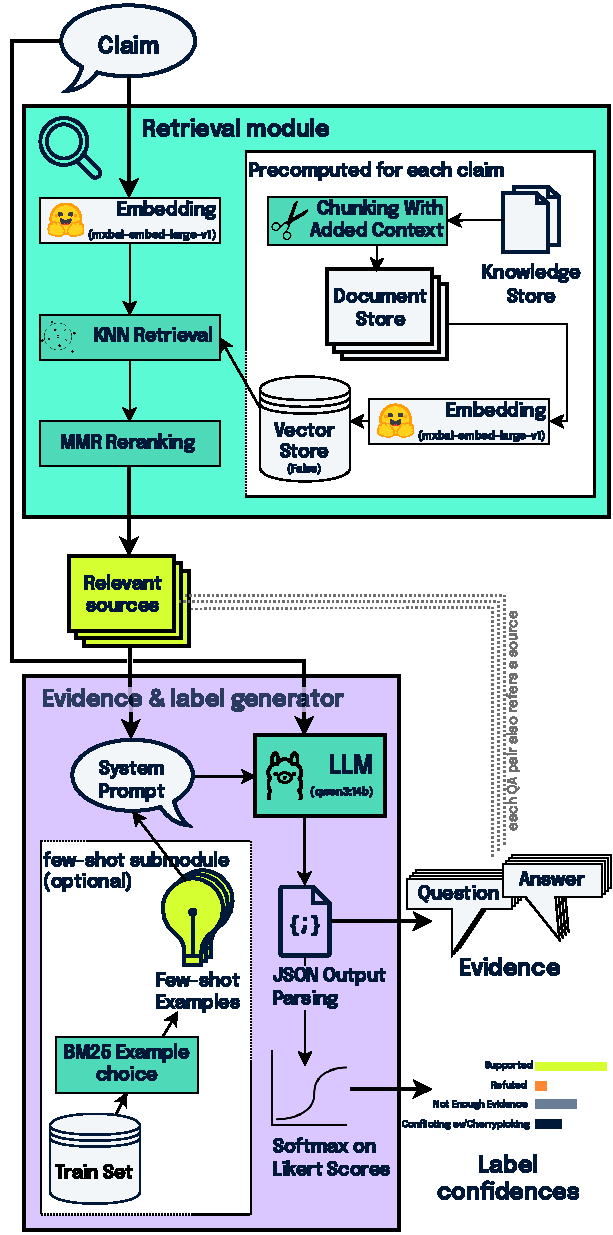
\includegraphics[width=0.6\textwidth]{figures/pipeline2025.pdf}
    \caption{Our refreshed fact-checking pipeline used in CTU AIC FEVER 8 submission, adapted from~\cite {ullrich-etal-2024-aic}.}
    \label{fig:pipeline2025}
\end{figure}


This paper introduces our system, discusses its design choices and how do they account on the score.
We suggest our system as the new strong baseline -- simple at core, competitive results -- providing the code and reproduction advice.


\section{System description}
\label{sec:system2025}

Our system is a straightforward adaptation of the AIC CTU Averitec system designed one year prior, published in~\cite{ullrich-etal-2024-aic}.
The cited paper describes the system in detail, with ablation studies and justifications of each step.
Our pipeline, depicted in Figure~\ref{fig:pipeline2025}, consists of precomputation, retrieval, and generation modules:

\begin{enumerate}[i.]  % First-level: i., ii., iii.
    \item Precomputation module
    \begin{enumerate}[1.]  % Second-level: 1., 2., 3.
        \item The provided AVeriTeC \textbf{knowledge store} \cite{averitec2024} is split into chunks of specified maximum length, each marked with metadata of its URL and the full texts of the chunk before and after.
        \item The chunks are then embedded into their vector representations, using only the chunk texts and no metadata.
        \item Out of all chunk embeddings, a \textbf{vector store} is produced for each claim to be stored as a vector database.
    \end{enumerate}
    \item Retrieval module
    \begin{enumerate}[1.]   % Second-level: 1., 2., 3.
        \item The \textbf{Claim} is embedded into its vector representation using the same model used in i.2.
        \item $k$ nearest neighbours are then retrieved from the vector store, along with their \textbf{chunk embeddings}
        \item The chunk embeddings are then re-ranked using the Maximal Marginal Relevance (MMR) method~\cite{carbonell-mmr}, maximizing the embedding distances between retrieval results while minimizing their distance to the claim.
        Ultimately, we output a subset of $l$~diverse \textbf{sources} for the claim ($l<k$), augmenting each with its context before, after, and the text of its URL.
    \end{enumerate}
    \item Evidence \& label generation module
    \begin{enumerate}[1.]   % Second-level: 1., 2., 3.
        \item We instruct a Large Language Model (LLM) to produce Question-Answer pairs required to fact-check given claim based on the provided sources, and predict its veracity verdict in a single output. We pass it the texts of all $l$ sources, and several few-shot QA-pair generation examples picked from Averitec train set retrieved using BM25 based on the tested claim. The whole instruction is serialized into a system prompt and the format we used can be seen in Appendix~\ref{appendix_sec:system_prompt}.
        \item \textbf{Claim} is then passed to the LLM as a user message.
        \item LLM is called to \textbf{generate the evidence} as a Question-Answer-Source triples and the Likert-scale scores for each possible \textbf{veracity verdict} in a single prediction, performing a chain of thought. 
        \item The LLM output is parsed, and the verdict with the highest score is chosen for the claim.
    \end{enumerate}
\end{enumerate}

The main differences between this year's AIC \averitec{} system, opposed to last year's AIC AVeriTeC system, are the omission of knowledge store pruning in the precomputation step\footnote{The precomputed vector stores were required to be independent on claim text in \averitec{}.}, and, importantly, the choice of LLM.
\subsection{Model and parameter choices}
\label{sec:choices}
To produce our submission in the \averitec{} shared task, the following choices were made to deploy the pipeline from section~\ref{sec:system2025}:

\texttt{mxbai-embed-large-v1}~\cite{li-li-2024-aoe,emb2024mxbai} is used for the vector embeddings, and the maximum chunk size is set to 2048 characters, considering its input size of 512 tokens and a rule-of-thumb coefficient of 4 characters per token to exploit the full embedding input size and produce the smallest possible vector store size without neglecting a significant proportion of knowledge store text.

\texttt{FAISS}~\cite{douze2024faiss,johnson2019billion} index is used as the vector database engine, due to its simplicity of usage, exact search feature and quick retrieval times (sub-second for a single \averitec{} test claim).

$l=10, k=40, \lambda=0.75$ are the parameters we use for the MMR reranking, meaning that 40 chunks are retrieved, 10 sources are yielded after MMR-diversification, and the tradeoff between their similarity to the claim and their diversity is 3:1 in favour of the source similarity to the claim (explained in more detail in~\cite{ullrich-etal-2024-aic}). 

\texttt{Ollama} wrapper around \texttt{llama.cpp} is the LLM engine we use to deploy LLMs within the \averitec~test environment due to its robustness and ease of deployment.

\texttt{Qwen3-14b}~\cite{yang2025qwen3technicalreport} is the LLM we use to produce the evidence and labels, we also let it generate its own \texttt{<think>} sequences, although further experimentation (Table~\ref{tab:ablation}) suggests that the thinking tokens may not justify the costs of their prediction, as they seem to perform on par with using only the evidence \& label LLM outputs for its chain of thought.

%!TEX ROOT=../emnlp2023.tex

\section{Results and analysis}
\label{nothink}


\begin{table}[h]
\centering
\begin{tabular}{l
>{\centering\arraybackslash}p{.7cm} 
>{\centering\arraybackslash}p{.7cm} 
>{\centering\arraybackslash}p{.7cm} 
>{\centering\arraybackslash}p{.7cm} 
>{\centering\arraybackslash}p{.7cm}}
{\small{\textbf{System}}} &
\rotatebox{70}{\textbf{\footnotesize{old AVeriTeC score}}} &
\rotatebox{70}{\textbf{Q only} {\footnotesize{(\evr)}}} &
\rotatebox{70}{\textbf{Q + A} {\footnotesize{(\evr)}}} &
\rotatebox{70}{\textbf{\footnotesize{new AVeriTeC score}}} &
\rotatebox{70}{{\footnotesize{\textbf{time per claim}}}} \\
\hline
{\small{AIC CTU}}       & 0.41 & 0.20 & \textbf{0.48} & \textbf{0.33} & 54\textit{s} \\
{\small{HUMANE}}        & 0.45 & 0.19 & 0.43 & 0.27 & 29\textit{s} \\
{\small{yellow flash}}  & 0.16 & 0.16 & 0.41 & 0.25 & 32\textit{s} \\
{\small{FZIGOT}}        & 0.46 & \textbf{0.36} & 0.40 & 0.24 & 19\textit{s} \\
{\small{EFC}}           & 0.49 & 0.13 & 0.35 & 0.20 & \textbf{~7\textit{s}} \\
{\small{checkmate}}     & 0.38 & 0.18 & 0.34 & 0.20 & 22\textit{s} \\
\hline
{\small{Baseline}}      & \textbf{0.50} & 0.27 & 0.34 & 0.20 & 34\textit{s} \\
\end{tabular}
\caption{\averitec{} shared task system leaderboard as shared by organizers, listing new \evr{}-recall-based~\cite{akhtar2024ev2r} and legacy hu-METEOR AVeriTeC scores. Evaluated using AVeriTeC 2025 test set. Best scores are bold.}
\label{tab:leaderboard}
\end{table}

In Table~\ref{tab:leaderboard}, we reprint the final test-leaderboard of \averitec{} shared task as provided by the organizers.
Our system introduced in Section~\ref{sec:system2025} scores first in the decisive metric for the task -- the new AVeriTeC score -- with a significant margin.
This came as a surprise to its authors, as neither the values of the old, hu-METEOR-based AVeriTeC score~\cite{averitec2024}, nor the dev-leaderboard available during system development phase (where our system scored 4th), suggested its supremacy.
Let us therefore proceed with a discussion of possible strengths that could have given our system an edge in verifying the \averitec{} test-set of previously unseen 1000 claims.

\subsection{Why does the system perform well?}
\label{sec:why}
So why should our system outperform the \averitec{} baseline and even the other systems submitted to \averitec{} shared task despite the simplicity of its design (Figure~\ref{fig:pipeline2025}) which boils down to a straightforward case of retrieval-augmented generation (RAG)?

The main reason, in our experience, is the large \textbf{context size} we opt for -- while even the \averitec{} baseline processes the claims and sources in a manner more sophisticated than we do, it processes the knowledge store on a \textit{sentence} level, reducing the amount of information passed to the LLM as opposed to working with \textit{documents} as a whole, which is the strategy our system approximates.

Despite our proposed integration of LLM into the pipeline being rather vanilla, combining sources of total length of as much as 60K characters\footnote{In other words, around 33 standard pages. This number follows from our parameter choices in Section~\ref{sec:choices}: 10 sources are retrieved for each claim, each with $\sim2048$ characters of the embedded text, and additional $\sim4096$ characters of context.} on model input yields highly competitive results, leveraging its own trained mechanisms of context processing.

Our other advantages may have been using a very recent model, Qwen3~\cite{yang2025qwen3technicalreport}, which naturally has a slightly higher leakage of 2025 claims into its train set than older models, and outperforms the previous LLM generations at long sequence processing. Furthermore, our pipeline design only uses a single LLM call per claim, meaning we could use the generously-sized 14B variant of Qwen3 and still match the time limit with Nvidia A10 and 23GB VRAM.

\subsection{Scoring change impact}
\label{sec:score}
While the new AVeriTeC score based on~\evr-recall~\cite{akhtar2024ev2r} estimates the proportion of correctly fact-checked claims\footnote{Claims with sound evidence w.r.t. human annotation, and an exact match in predicted label.} in all claims, just like the old hu-METEOR-based AVeriTeC score did, their underlying methods differ.
Most importantly, an LLM-as-a-judge approach is now used instead of symbolic evidence comparison method.
The rise of our system from 3rd place in AVeriTeC shared task~\cite{schlichtkrull-etal-2024-automated} to 1st place in~\averitec{} without any major system change\footnote{Despite scaling down.} can therefore also be attributed to the used scoring method.
The old scoring method was, for example, found to be prone to some level of noise, as it was not robust against evidence duplication~\cite{malon-2024-multi}, which was a found exploit to boost evidence recall.

The discrepancy between old and new AVeriTeC score in Table~\ref{tab:leaderboard} could motivate a further study on how the new score behaves, for example using the test-prediction files from last year AVeriTeC shared task systems.
The familiarity of the systems, the availability of their hu-METEOR scores and documentation, may reveal valuable insights into the \evr{} evaluation method itself, as in which behaviours does it punish and reward.

\subsection{LLM impact}
\label{llmimp}
\begin{table}[h]
\centering
\begin{tabular}{l
>{\centering\arraybackslash}p{1cm} 
>{\centering\arraybackslash}p{1cm} 
>{\centering\arraybackslash}p{1cm}}
\textbf{LLM} &
\rotatebox{70}{\textbf{Q only} {\footnotesize{(\evr)}}} &
\rotatebox{70}{\textbf{Q + A} {\footnotesize{(\evr)}}} &
\rotatebox{70}{\textbf{\footnotesize{new AVeriTeC score}}} \\
\hline
GPT-4o\textsubscript{\texttt{2024-05-13}}      & 0.30 & 0.58 & 0.40 \\
Llama3.1-70B& 0.37 & 0.54 & 0.39 \\
qwen3:14B\textsubscript{\texttt{/no\_think}}     & 0.29 & 0.59 & 0.41 \\
qwen3:14B\textsubscript{\texttt{/think}}        & 0.20 & 0.59 & 0.42 \\
\hline
\end{tabular}
\caption{Ablation study on LLM choice and \texttt{<think>}-tokens impact on \averitec{} dev-score. Pipeline design (Figure~\ref{fig:pipeline2025}), retrieval results, system and user prompts are fixed. Evaluated using an on-premise~\evr{} scorer with Ollama-hosted Llama3.3-70B as a judge.}
\label{tab:ablation}
\end{table}

In 2024, we have experimented with then available versions of GPT-4o and Llama3.1-70B and found the open-source Llama to perform encouragingly well, depite the still-quite-cumbersome model size and the need for its quantization~\cite{ullrich-etal-2024-aic}.
This year, we have simply gone for the most recent open-weights LLM at the largest parameter count we could fit within our \averitec{} compute budget, thus choosing the Qwen3 at its 14B parameter size~\cite{yang2025qwen3technicalreport}.

Qwen3 was trained to produce thinking tokens by default, an approach popularized by DeepSeek~\cite{deepseekai2025deepseekr1incentivizingreasoningcapability} and OpenAI research models, to force the chain of thought.
We have experimented with enabling and disabling this feature to see if it has an impact on the AVeriTeC score, and compared the model output quality to our last year prediction dumps, with evaluation experiments listed in Table~\ref{tab:ablation}.

Both Qwen3 evidence and label generation settings perform on par with previous GPT-4o generation, which validates our model choice.
The thinking tokens, while producing legitimate-looking writeups of the fact-checking workflows (see Appendix~\ref{appendix_sec:think}) were not shown to stimulate an improvement in AVeriTeC score in the ablation study (Table~\ref{tab:ablation}), so we suggest to disable this feature in future reproductions in favour of a faster prediction time (54s in the Table~\ref{tab:leaderboard} was produced with the thinking feature \textit{enabled}, so disabling it might solve the issue with near-limit runtime our pipeline suffers from). 


\section{Conclusion}
In this paper, we have introduced our simple yet efficient RAG system which performed competitively well under time and compute constraints in \averitec{} shared task, in May 2025.
We release the used code along with usage instructions for producing the~\averitec{} submission, vector stores needed for the pipeline to run and their build scripts at 
\url{https://github.com/heruberuto/FEVER-8-Shared-Task/}
which is a fork of the \averitec{} baseline repository.

We attribute our success mostly to the use of \textit{document} rather than \textit{sentence} level of retrieval granularity and an employment of a recent LLM at a size which utilizes the whole compute and time budget with only around 10\% time reserve as a failsafe.
We encourage further usage of our system as a strong and easy-to-setup baseline for further research in automated fact checking and will be happy to answer any questions on the referred contacts.

\subsection{Future works}
\begin{enumerate}
    \item Integrate a live search API as in~\cite{malon-2024-multi} as a retriever into the AIC pipeline (Figure~\ref{fig:pipeline2025}) to achieve a real-world generalization
    \item Section~\ref{sec:score} suggests to look at the key differences between legacy and \evr{} scoring methods in terms of the available 2024 AVeriTeC leaderboard and available model documentations -- we believe this could reveal valuable hints both scoring and pipelinne improvements in future work
\end{enumerate}
%!TEX ROOT=../ctutest.tex

\chapter{Conclusion}
\label{chap:conclusion}
In this study, I have presented my current challenges and their motivation -- a desire for an automated scheme to assist fact-checking.
The solutions are being proposed in other literature and rely mostly on transformers, which is the current state of the art for nearly every NLP task.
The transformer usage paradigm is shifting (from the approach of \textit{fine-tuning} a \textit{pre-trained} transformer to \textit{prompting} or \textit{few-shotting} a Large Language Model), which will impact my dissertation and also yield new challenges in modernizing our previous work.

So far, numerous datasets, most notably the \FCZ and \CTK, have been collected, a working fact-checking pipeline was deployed on them, and the models we trained were published for further use.

Other tasks are to be established among the scientific public, importantly the claim generation and its model-based metrics, ongoing research such as the claim generation model training, collection of additional data in Czech, English, Polish, and Slovak is to be concluded, and new solutions for the whole problem of automated fact-checking are to be proposed, utilizing the new SOTA methods, such as the Large Language Models.

The point of the precedent chapters of the study was to give insights on what has been done so far, what is its value, what is the context in which this is happening, and what are the likely next steps in the future of my research.

%\bibliographystyle{amsalpha}
\bibliographystyle{apalike}
\bibliography{dissertation}
\appendix
%\chapter{Czech-English data translations}
\section{Translated figures}

\begin{figure}[H]
\centering
 \fbox{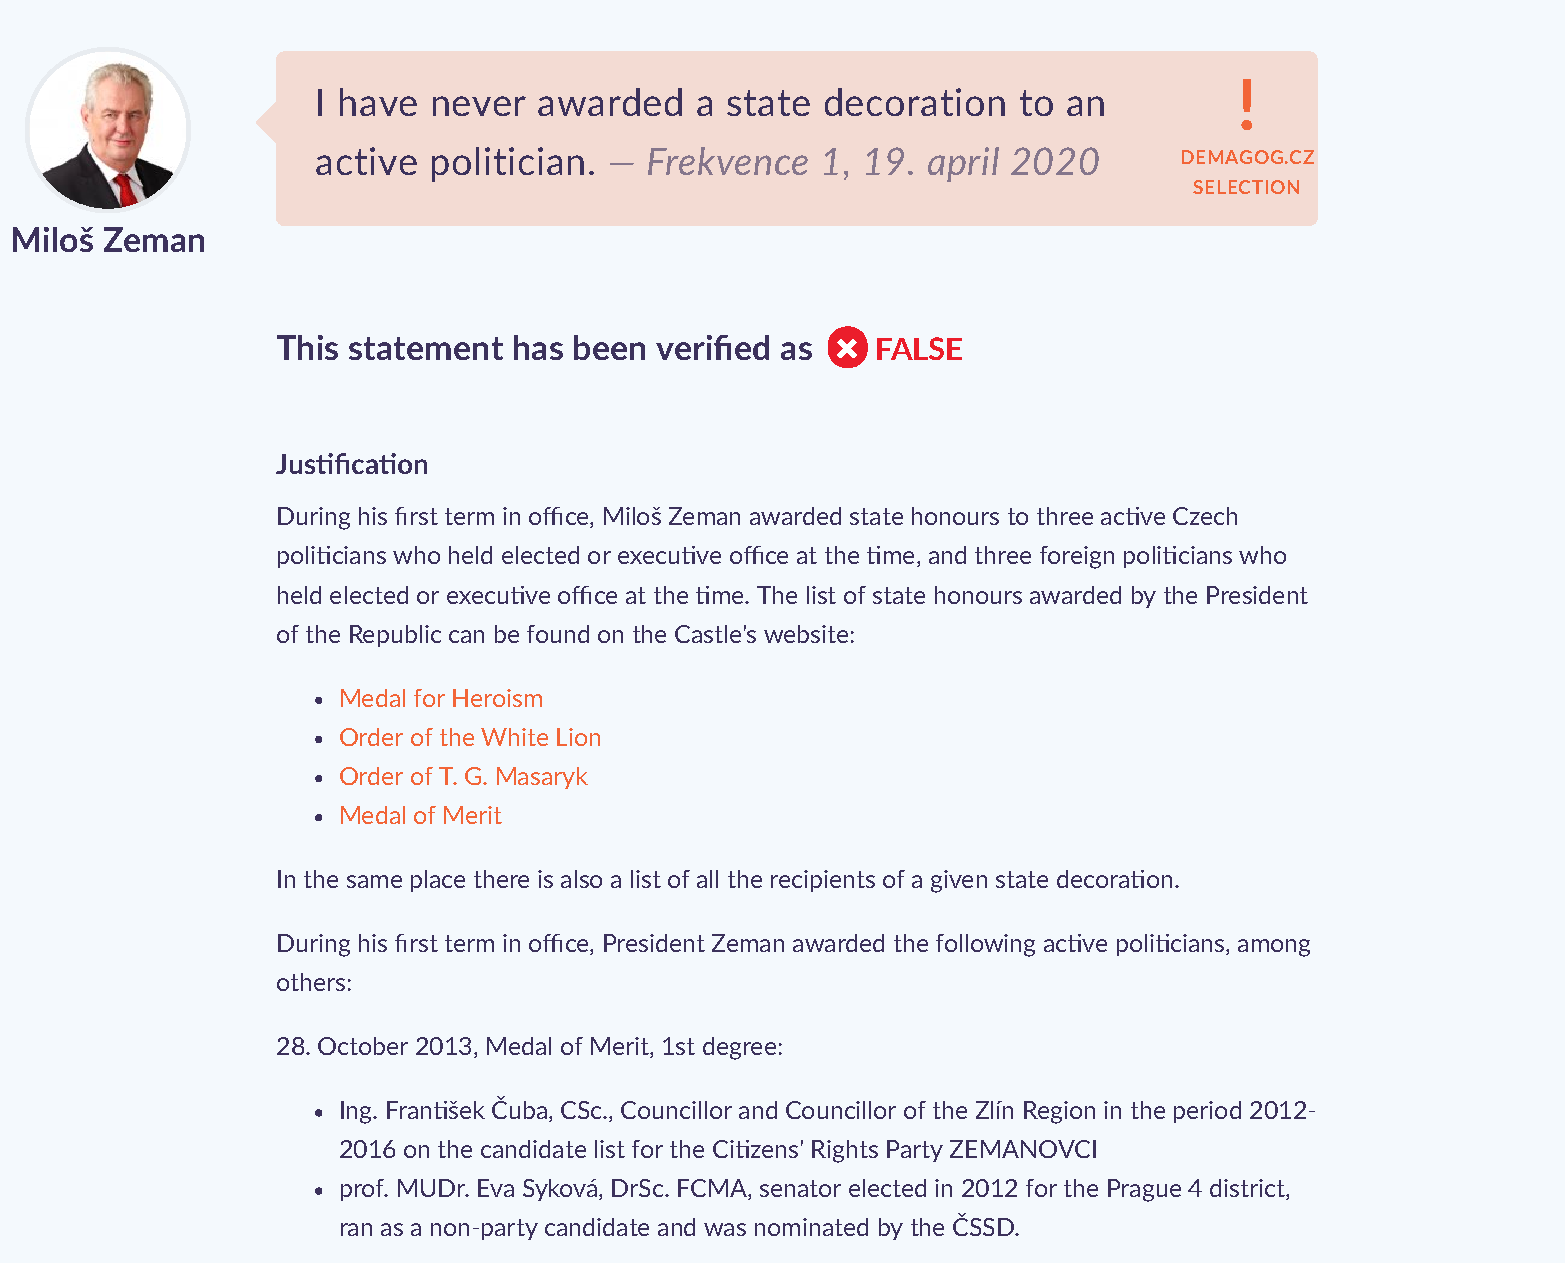
\includegraphics[width=\textwidth]{fig/demagog_en.pdf}}
\caption[English Translation of Figure~\ref{fig:demagog}]{Translated fact verification from Czech portal \textsf{Demagog.cz} -- original in Figure~\ref{fig:demagog}}
\label{trans:demagog}
\end{figure}

\begin{figure}
\thisfloatpagestyle{empty}
\vspace{-2cm}
 \makebox[\textwidth][c]{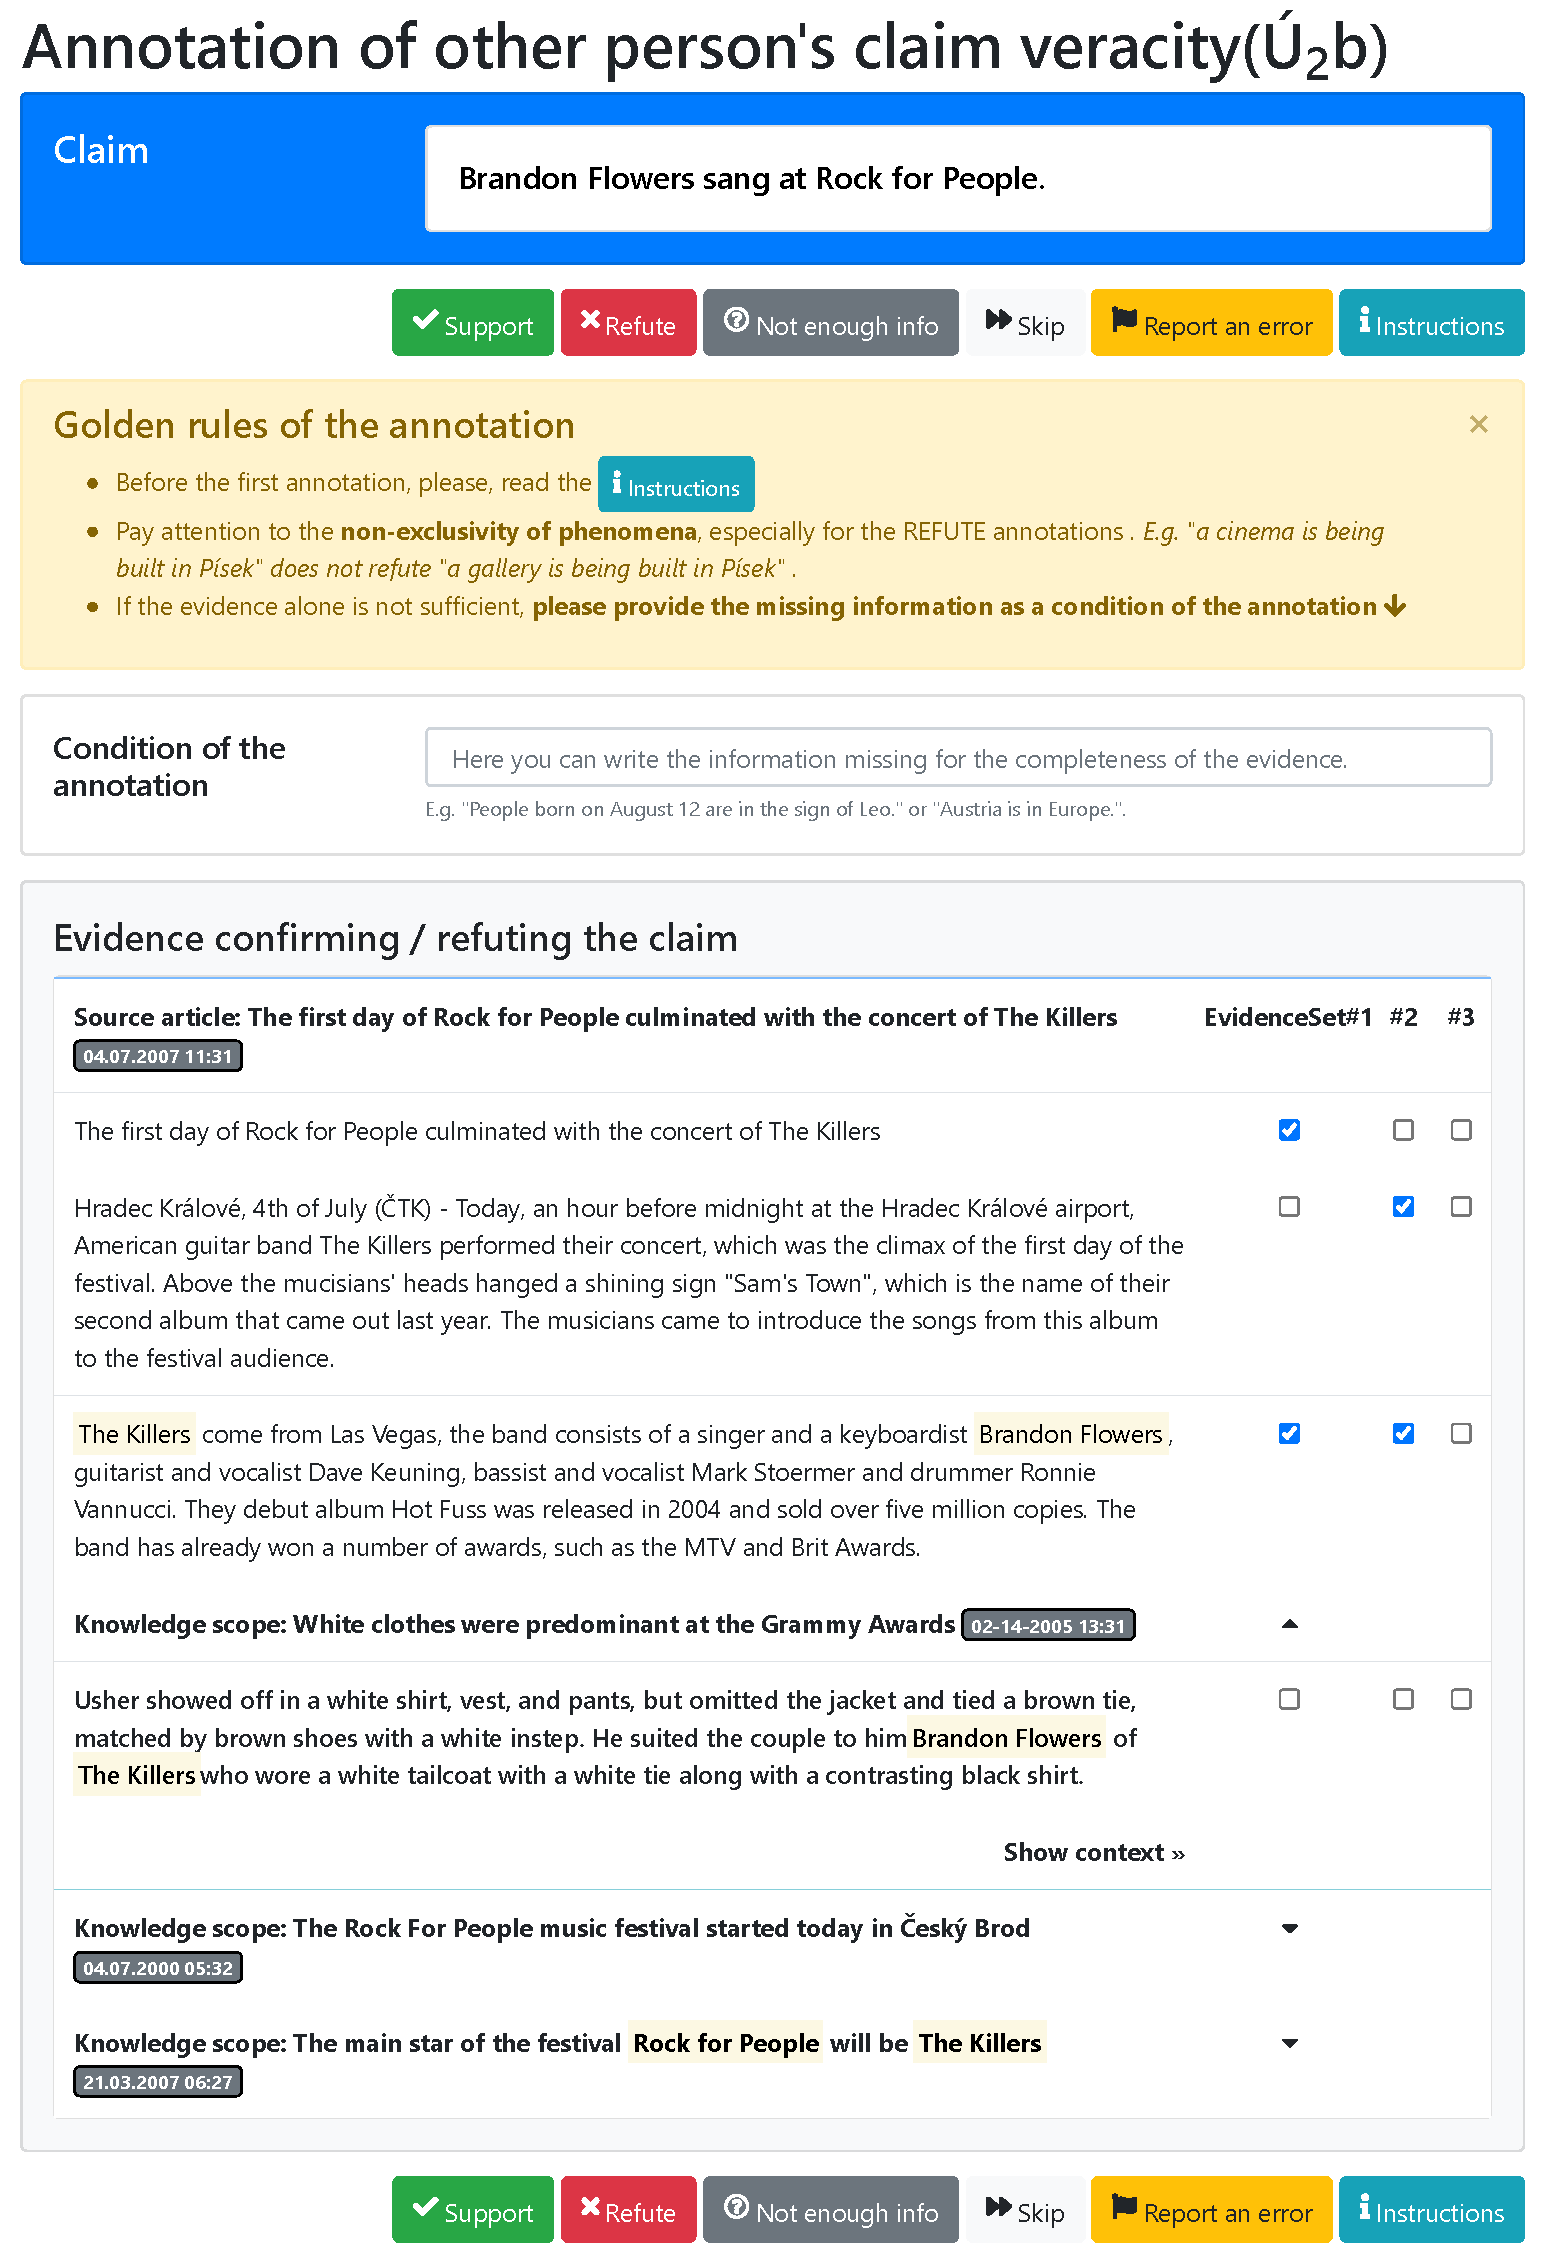
\includegraphics[width=18cm]{fig/annotation_en.pdf}}
\caption[English Translation of Figure~\ref{fig:annotation}]{The labelling interface of \textsf{FCheck} platform. Czech original in Figure~\ref{fig:annotation}}
\label{trans:annotation}
\end{figure}

\chapter{Acronyms}
\begin{description}
\item[BERT] Bidirectional Encoder Representations from Transformers
\item[GPT] Generative Pre-trained Transformer 
\item[FEVER] Fact Extraction and Verification -- series of Shared tasks focused on fact-checking
\item[IR] Information Retrieval
\item[SOTA] State of the Art
\item[XSum] Extreme Summarization -- summarizing article into one sentence
\item[NLI] Natural Language Inference
\item[ČTK] Czech Press Agency
\end{description}


\end{document}